% =====================================================================
% Previsão da Carga de Casos do Programa Bolsa Família:
% redes neurais do zero, covariáveis de demografia e emprego, um
% benchmark fora do tempo e uma projeção até 2028.
%
% Working Paper #10
% Autores: Leonardo Chalhoub, Alexandre Maciel Rolim,
%          Luis Fernando Kranz, Jefferson Korte
% Compilação: pdflatex articles/bolsa-familia-previsao.tex (2x)
% =====================================================================

\documentclass[12pt,a4paper,oneside]{article}

\usepackage[T1]{fontenc}
\usepackage[utf8]{inputenc}
\usepackage[brazilian]{babel}
\usepackage{amsmath}
\usepackage{amssymb}
\usepackage{bm}
\usepackage{newtxtext}
\usepackage{newtxmath}
\usepackage[section]{placeins}
\usepackage[a4paper,top=3cm,bottom=2cm,left=3cm,right=2cm]{geometry}
\usepackage{setspace}
\usepackage{indentfirst}
\usepackage{titlesec}
\usepackage{caption}
\usepackage{booktabs}
\usepackage{array}
\usepackage{multirow}
\usepackage{siunitx}
\usepackage{graphicx}
\usepackage[colorlinks=true,
            urlcolor=blue!60!black,
            linkcolor=black,
            citecolor=black,
            breaklinks=true]{hyperref}
\usepackage{url}
\usepackage{xurl}
\Urlmuskip=0mu plus 1mu\relax
\usepackage{float}
\usepackage{tcolorbox}

\graphicspath{{figures-pbf-forecast/}}

\onehalfspacing
\setlength{\parindent}{1.25cm}
\setlength{\parskip}{0pt}

\titleformat{\section}{\normalfont\bfseries\large\uppercase}{\thesection}{0.6em}{}
\titleformat{\subsection}{\normalfont\bfseries\normalsize}{\thesubsection}{0.6em}{}
\titlespacing*{\section}{0pt}{18pt}{8pt}
\titlespacing*{\subsection}{0pt}{12pt}{6pt}

\captionsetup[table]{labelfont=bf,name=Tabela,labelsep=endash,
                     position=above,justification=centering,font=small}
\captionsetup[figure]{labelfont=bf,name=Figura,labelsep=endash,
                      position=below,justification=centering,font=small}
\captionsetup{skip=6pt}

\sisetup{group-separator={.},group-minimum-digits=4,output-decimal-marker={,}}

\newcounter{mref}
\newcommand{\refentry}[1]{%
  \par\smallskip\noindent\hangindent=1.25cm\hangafter=1
  [\refstepcounter{mref}\themref\label{#1}]\ \ignorespaces}
\newcommand{\C}[1]{[\ref{#1}]}

% Stamp de compilação injetado pelo CI (deploy-pages.yml).
% Para builds locais, este arquivo default é usado — basta um pdflatex direto
% e a capa exibe "(dev local)". Em CI, este arquivo é sobrescrito antes da
% compilação com timestamp BRT + SHA do commit que disparou o deploy.
\newcommand{\COMPILESTAMP}{compila\c{c}\~ao local}
\newcommand{\COMPILESHA}{dev}


\begin{document}

% ---------- CAPA ---------------------------------------------------------
\begin{titlepage}
  \begin{center}
    \vspace*{1.0cm}
    {\small\textsc{Artigo de pesquisa \quad\textbar\quad Aprendizado de Máquina \textendash{} Previsão de Séries Temporais}}\\
    {\small Working Paper \#10 \textemdash{} Versão 1.0 \textemdash{} Junho de 2026}\\[2pt]
    {\footnotesize Compilada em \COMPILESTAMP\ \textbullet\ \texttt{\COMPILESHA}}

    \vfill

    {\LARGE\bfseries
     PREVISÃO DA CARGA DE CASOS\\[6pt]
     DO PROGRAMA BOLSA FAMÍLIA}\\[14pt]

    {\large
      \textit{Redes neurais construídas do zero, covariáveis de\\
      demografia e emprego, um benchmark fora do tempo\\
      e uma projeção até 2028}}

    \vfill

    {\large\bfseries Leonardo Chalhoub \quad\textbullet\quad Alexandre Maciel Rolim}\\[4pt]
    {\large\bfseries Luis Fernando Kranz \quad\textbullet\quad Jefferson Korte}\\[10pt]
    \begin{minipage}{0.90\textwidth}\centering\footnotesize
      Todos os autores atuam como \textbf{pesquisadores independentes}, Brasil.\\[4pt]
      \textit{Leonardo Chalhoub} \textemdash{} \textit{Expert Data Engineer}; Mestre em
      Administração (Finanças), UFRGS; graduando em Engenharia de Software,
      Universidade Estácio de Sá. Rio de Janeiro, RJ. ORCID: 0000-0003-0484-158X.\\[2pt]
      \textit{Alexandre Maciel Rolim} \textemdash{} Tecnólogo em Radiologia; Mestre em
      Proteção Radiológica, IFSC. Florianópolis, SC. ORCID: 0009-0000-3983-4713.\\[2pt]
      \textit{Luis Fernando Kranz} \textemdash{} Tecnólogo em Radiologia; Mestre em
      Administração, UFRGS. Porto Alegre, RS. ORCID: 0009-0009-6015-3141.\\[2pt]
      \textit{Jefferson Korte} \textemdash{} Estudante de Ciência da Computação, UTFPR.
      Curitiba, PR. ORCID: 0009-0006-9466-9830.\\[4pt]
      \textbf{Correspondência:} Leonardo Chalhoub \textbullet{} \texttt{leochalhoub@hotmail.com}
    \end{minipage}

    \vfill

    \begin{minipage}{0.86\textwidth}\centering\small
      \textit{Quantos núcleos familiares o maior programa de transferência
      condicionada de renda da América Latina atenderá nos próximos anos, e o
      que governa essa demanda? Tratamos a \emph{carga de casos} (o número de
      famílias beneficiárias) como uma série temporal em painel e a prevemos
      com redes neurais implementadas inteiramente do zero em C++17. Sobre
      \num{5542} municípios e 156 meses (2013\textendash 2025), comparamos
      modelos \emph{univariados} (apenas o próprio histórico) a modelos
      \emph{multivariados} alimentados por covariáveis anuais de população
      (IBGE) e de emprego formal (RAIS), sob avaliação rigorosa fora do tempo,
      e projetamos a trajetória nacional até dezembro de 2028. Dois achados
      organizam o artigo: a profundidade só compensa quando a estrutura do
      sinal a recompensa; e as covariáveis de demografia e mercado de trabalho
      carregam sinal real, cujo valor cresce com o horizonte de previsão.}
    \end{minipage}

    \vspace{0.8cm}
  \end{center}
\end{titlepage}

% ---------- RESUMO ABNT --------------------------------------------------
\begin{center}
{\bfseries RESUMO}
\end{center}

\noindent
Este artigo formula a previsão da carga de casos do Programa Bolsa
Família \textemdash{} o número de famílias beneficiárias \textemdash{}
como um problema de previsão de séries temporais em painel e o resolve
com redes neurais construídas inteiramente do zero em C++17, sem
bibliotecas de aprendizado profundo. A partir de uma camada bruta de
\num{2533885299} pagamentos do Portal da Transparência da
Controladoria-Geral da União (CGU), mineramos um painel
município~$\times$~mês com \num{5542} municípios e 156 meses
(2013\textendash 2025) e o enriquecemos com duas covariáveis anuais
\textemdash{} população residente (IBGE) e emprego formal ativo
(RAIS/PDET) \textemdash{}, reconciliadas ao código municipal do painel por
um \emph{crosswalk} com 99,5\% de cobertura. Treinamos um único modelo
global e o avaliamos sob protocolo honesto: padronização com meses de
treino apenas (sem vazamento), covariáveis defasadas (sem peeking),
partição \emph{fora do tempo} (alvos anteriores a janeiro de 2025
treinam; janeiro a dezembro de 2025 testam, $\approx$\num{66504} previsões
por horizonte) e linha de base ingênua forte (persistência). Comparamos
cinco modelos \textemdash{} persistência, autorregressão linear,
perceptron multicamadas profundo ($14\to 64\to 32\to 1$) e as versões
\emph{com covariáveis} de ambos ($16\to\cdots$) \textemdash{} em quatro
horizontes ($H\in\{1,3,6,12\}$ meses) com MAE, MAPE, RMSE e $R^2$, e
inferimos significância por bootstrap pareado, teste de Wilcoxon e taxa de
vitória. Achados: (i) a um mês a carga de casos é quase um passeio
aleatório e nenhum modelo aprendido supera a persistência; (ii) em
horizontes de planejamento (6 meses) a autorregressão reduz o MAE em
27\% sobre a ingênua, com vantagem grande e robusta; (iii) a profundidade
é \emph{dominada} pela autorregressão em todo horizonte, mesmo com
covariáveis; (iv) as covariáveis de demografia e emprego carregam sinal
real cujo valor \emph{cresce com o horizonte}: irrelevantes ou prejudiciais
a curto prazo, elevam o modelo linear em 12 meses de $+10\%$ para
$+17\%$ de redução de MAE, tornando o modelo linear com covariáveis o
melhor preditor de longo prazo; (v) a projeção nacional indica que a carga
de casos atingiu o pico em 2022\textendash 2023 e recua, com erro agregado
de backtest inferior a 4,7\% em 12 meses. Documentamos ainda uma forte
relação estrutural entre cobertura do programa e intensidade de emprego
formal nos municípios (correlação log-log de $-0{,}66$ em 2024).
Conclui-se que a demanda estrutural é plana ou declinante e que o custo
futuro é governado pelo \emph{valor} do benefício \textemdash{} uma
escolha de política \textemdash{}, não por uma carga de casos em expansão.

\medskip

\noindent\textbf{Palavras-chave}: previsão de séries temporais; redes
neurais artificiais; perceptron multicamadas; covariáveis exógenas;
Programa Bolsa Família; emprego formal; RAIS; demografia; avaliação fora
do tempo; C++.

\bigskip

\begin{center}
{\bfseries ABSTRACT}
\end{center}

\noindent
This paper frames forecasting the Bolsa Família caseload \textemdash{}
the number of beneficiary families \textemdash{} as a panel time-series
problem and solves it with neural networks built entirely from scratch in
C++17. From a bronze layer of \num{2533885299} payment records (CGU), we
mine a municipality~$\times$~month panel of \num{5542} municipalities and
156 months (2013\textendash 2025) and enrich it with two annual
covariates \textemdash{} resident population (IBGE) and active formal
employment (RAIS) \textemdash{} reconciled to the panel's municipal code
by a crosswalk covering 99.5\% of municipalities. A single global model is
trained and evaluated honestly: leakage-free standardisation, lagged
covariates, an out-of-time split (targets before January 2025 train;
January to December 2025 test, $\approx$66{,}504 forecasts per horizon),
and a strong naive baseline. We compare five models \textemdash{}
persistence, a linear autoregression, a deep MLP, and the
covariate-augmented versions of both \textemdash{} across four horizons,
with significance from paired bootstrap, Wilcoxon tests and win rates. We
find that at one month no learned model beats persistence; at planning
horizons the linear autoregression cuts MAE by 27\% over naive; depth is
dominated by the linear model everywhere, even with covariates; and the
covariates carry real signal whose value grows with the horizon \textemdash{}
negligible or harmful in the short run, they lift the 12-month linear model
from $+10\%$ to $+17\%$ MAE reduction. The national projection shows the
caseload peaked in 2022\textendash 2023 and is declining, with aggregate
backtest error below 4.7\% at twelve months. We also document a strong
structural relationship between program coverage and formal-employment
intensity across municipalities (log-log correlation $-0.66$ in 2024). We
conclude that structural demand is flat-to-falling, so future cost is
governed by the benefit level \textemdash{} a policy choice.

\medskip

\noindent\textbf{Keywords}: time-series forecasting; artificial neural
networks; multilayer perceptron; exogenous covariates; Bolsa Família;
formal employment; out-of-time evaluation; C++.

\newpage
\tableofcontents
\newpage

% =====================================================================
\section{Introdução}
% =====================================================================

A pergunta que este artigo responde é operacional e mensurável:
\emph{dado o histórico do maior programa de transferência condicionada de
renda da América Latina, qual é a projeção mais defensável do número de
famílias beneficiárias nos próximos anos, com que acurácia tal previsão
pode ser feita, e que informação \textemdash{} o próprio passado da série,
a demografia, o mercado de trabalho \textemdash{} de fato a melhora?} A
resposta tem implicação direta de política pública, porque o custo total
de um programa de transferência de renda é, em primeira aproximação, o
produto de duas grandezas:
\begin{equation}
\text{custo} \;\approx\; \underbrace{\text{carga de casos}}_{\text{demanda estrutural}}
\;\times\;
\underbrace{\text{benefício médio}}_{\text{alavanca de política}} .
\label{eq:custo}
\end{equation}
O valor do benefício é uma \emph{escolha} discricionária do gestor; a
carga de casos \textemdash{} \emph{caseload}, o número de núcleos
familiares na folha de pagamento \textemdash{} é demanda estrutural,
governada por dinâmicas demográficas, de mercado de trabalho e de
elegibilidade que nenhum decreto altera no curto prazo. Uma previsão
crível da carga de casos isola a parcela do gasto futuro que \emph{não} é
decisão discricionária. É essa parcela que tratamos aqui.

A escolha de objeto não é trivial. Diferentemente do gasto nominal
\textemdash{} que exige deflação e mistura mudanças de preço e de
quantidade \textemdash{}, a contagem de famílias é uma grandeza física,
robusta a regimes institucionais e que não requer correção monetária. É a
base limpa sobre a qual qualquer projeção de custo deve ser erguida. E,
por ser uma série genuína \textemdash{} com tendência, sazonalidade e
forte autocorrelação \textemdash{}, é também um banco de provas ideal para
duas perguntas metodológicas de interesse independente: \emph{quando a
profundidade compensa?} e \emph{quanto valem covariáveis exógenas de
contexto, e em que horizonte?}

\subsection{Contribuições}

Este trabalho oferece cinco contribuições.

\textbf{Primeira, empírica.} Construímos, de uma camada bruta de
\num{2533885299} registros, um painel município~$\times$~mês de
\num{5542} municípios e 156 meses (2013\textendash 2025) e produzimos com
ele uma projeção da carga de casos até dezembro de 2028 cuja incerteza é
quantificada por reamostragem fora do tempo, e não assumida.

\textbf{Segunda, de integração de dados.} Enriquecemos o painel com duas
covariáveis municipais anuais \textemdash{} população (IBGE) e emprego
formal ativo (RAIS/PDET) \textemdash{}, reconciliando três sistemas de
codificação municipal distintos (SIAFI, IBGE de 7 e de 6 dígitos) por um
\emph{crosswalk} de 99,5\% de cobertura, e descrevemos a relação
estrutural entre cobertura do programa e mercado de trabalho.

\textbf{Terceira, metodológica.} Implementamos as redes \emph{do zero} em
C++17 \textemdash{} inicialização de He, ReLU, retropropagação manual,
AdamW \textemdash{} sem qualquer biblioteca de aprendizado profundo,
seguindo o roteiro de \textsc{Chen} e \textsc{Gupta}~\C{ref:chen-gupta}.
Cada operação aritmética é auditável.

\textbf{Quarta, inferencial.} Submetemos toda comparação a protocolo
\emph{honesto}: padronização sem vazamento, covariáveis defasadas,
partição estritamente fora do tempo, e significância por bootstrap,
Wilcoxon e taxa de vitória município a município, reconhecendo que, com
$n\approx\num{66504}$ por horizonte, um valor-$p$ isolado é
desinformativo.

\textbf{Quinta, conceitual.} Documentamos dois fatos: a \emph{autorregressão
linear domina a rede profunda} em todo horizonte, mesmo alimentada com
covariáveis; e as covariáveis carregam sinal \emph{cujo valor cresce com o
horizonte} \textemdash{} negligível a um mês, decisivo a doze. O modelo do
tamanho certo, com a informação certa, generaliza melhor que o modelo de
maior capacidade.

\subsection{Organização}

A Seção~\ref{sec:contexto} situa o programa e a carga de casos. A
Seção~\ref{sec:dados} descreve as três fontes de dados, o \emph{crosswalk}
municipal e um panorama descritivo das relações entre caseload, população
e emprego. A Seção~\ref{sec:pipeline} apresenta os materiais e métodos de
engenharia de dados \textemdash{} o pipeline, a governança e a
reprodutibilidade. A Seção~\ref{sec:fundamentos} revisa os fundamentos de
previsão e de redes neurais. A Seção~\ref{sec:tarefa} formaliza a tarefa e o
protocolo. A Seção~\ref{sec:modelos} deriva os cinco modelos, com toda a
matemática. A Seção~\ref{sec:metricas} define métricas e inferência. As
Seções~\ref{sec:resultados} a~\ref{sec:significancia} apresentam a
acurácia, o efeito das covariáveis e sua significância. A
Seção~\ref{sec:interpretacao} interpreta \emph{quando} a profundidade e as
covariáveis ajudam. A Seção~\ref{sec:projecao} traz a projeção
2026\textendash 2028. As Seções~\ref{sec:limitacoes}
a~\ref{sec:conclusoes} discutem limitações, extensões e conclusões.

% =====================================================================
\section{O programa e a carga de casos}
\label{sec:contexto}
% =====================================================================

O Programa Bolsa Família foi instituído pela Lei n.\textsuperscript{o}
10.836, de 9 de janeiro de 2004~\C{ref:lei-pbf}, unificando programas de
transferência de renda anteriores em uma transferência condicionada à
frequência escolar e ao acompanhamento de saúde. Entre 2021 e 2023 passou
por duas reconfigurações: foi substituído pelo Auxílio Brasil (Medida
Provisória n.\textsuperscript{o} 1.061/2021, convertida na Lei
n.\textsuperscript{o} 14.284, de 29 de dezembro de 2021~\C{ref:lei-ab}) e
retornou como Bolsa Família (Medida Provisória n.\textsuperscript{o}
1.164/2023, convertida na Lei n.\textsuperscript{o} 14.601, de 19 de junho
de 2023~\C{ref:lei-nbf}). Essas transições alteraram regras e
nomenclatura, mas a grandeza que rastreamos \textemdash{} o número de
famílias na folha mês a mês \textemdash{} permanece comparável por ser
contagem física, não valor monetário. A Figura~\ref{fig:serie} exibe as
três faixas institucionais sobre a série completa.

A \emph{carga de casos} é a contagem de núcleos familiares distintos que
recebem ao menos uma parcela em um mês de competência \textemdash{} uma
medida de \emph{demanda atendida}, que combina demanda potencial,
capacidade administrativa de cadastro e política de revisão de
elegibilidade. Sua dinâmica responde a forças lentas \textemdash{}
transições no mercado de trabalho, fluxos do Cadastro Único,
recadastramentos \textemdash{} e a choques institucionais discretos. Essa
combinação de inércia forte com saltos ocasionais torna a série ao mesmo
tempo previsível em horizontes curtos e vulnerável a rupturas que nenhum
modelo univariado pode antecipar (Seção~\ref{sec:limitacoes}).

A leitura econômica da equação~\eqref{eq:custo} orienta o artigo: se a
carga de casos for plana ou declinante, a trajetória do custo é governada
pela alavanca de política, não pela demanda. Estabelecer empiricamente em
que regime a série se encontra \textemdash{} crescimento, platô ou recuo
\textemdash{} é insumo direto para o planejamento orçamentário.

% =====================================================================
\section{Dados}
\label{sec:dados}
% =====================================================================

\subsection{Três fontes}

O estudo cruza três bases públicas oficiais (Tabela~\ref{tab:dados}). A
primeira é a camada bruta de pagamentos do Bolsa Família do Portal da
Transparência da CGU~\C{ref:portal-transparencia}, com grão de
pagamento~$\times$~mês e \num{2533885299} registros, da qual mineramos a
carga de casos municipal,
\begin{equation}
f_{c,t} \;=\; \bigl|\{\,\text{NIS favorecidos distintos em } (c,t)\,\}\bigr|,
\end{equation}
para cada município $c$ e mês $t$. A segunda é a estimativa anual de
população residente por município do IBGE~\C{ref:ibge-pop}. A terceira é a
Relação Anual de Informações Sociais (RAIS), do Programa de Disseminação
das Estatísticas do Trabalho (PDET/MTE)~\C{ref:rais}, de onde extraímos o
estoque municipal de vínculos formais ativos por ano.

\begin{table}[H]
\centering
\caption{Fontes, grão e cobertura}
\label{tab:dados}
\small
\begin{tabular}{@{}lllr@{}}
\toprule
\textbf{Fonte} & \textbf{Conteúdo} & \textbf{Grão} & \textbf{Registros} \\
\midrule
CGU \textendash{} Portal da Transparência & pagamentos PBF & pagamento $\times$ mês & \num{2533885299} \\
\quad$\hookrightarrow$ painel derivado     & carga de casos & município $\times$ mês & \num{848526} \\
IBGE                                       & população residente & município $\times$ ano & \num{66840} \\
RAIS \textendash{} PDET/MTE                 & vínculos formais ativos & município $\times$ ano & \num{83537} \\
\bottomrule
\end{tabular}
\par\smallskip
{\footnotesize Fontes oficiais. O painel PBF cobre 156 meses
(2013\textendash 2025); as covariáveis, 2010\textendash 2024.}
\end{table}

\subsection{Reconciliação de códigos municipais}

As três fontes usam codificações municipais distintas: o painel da CGU
identifica municípios pelo código SIAFI de 4\textendash 6 dígitos; o IBGE,
pelo código de 7 dígitos; a RAIS, pelo código de 6 dígitos (IBGE sem o
dígito verificador). Construímos um \emph{crosswalk} SIAFI~$\to$~IBGE por
correspondência de \emph{(UF, nome do município normalizado)} \textemdash{}
removendo acentuação, caixa e pontuação \textemdash{}, e ligamos o código
de 6 dígitos da RAIS truncando o de 7 do IBGE. A correspondência cobre
\num{5542} de \num{5571} municípios (99,5\%); os 29 sem casamento
\textemdash{} em geral grafias divergentes \textemdash{} são excluídos da
amostra multivariada. Para que os modelos univariado e multivariado sejam
comparados sobre exatamente os mesmos exemplos, \emph{toda} a análise
restringe-se aos municípios com covariáveis disponíveis.

\subsection{Panorama descritivo}

Antes de modelar, vale ver o que os dados dizem. A
Figura~\ref{fig:contexto} indexa as três séries nacionais a 2013: a carga
de casos oscila com a política (salta na pandemia, recua na revisão dos
cadastros), enquanto população e, sobretudo, emprego formal seguem
trajetórias mais suaves e ascendentes. A Figura~\ref{fig:cobertura}
converte isso em uma \emph{taxa de cobertura} nacional (famílias por 100
habitantes), que subiu, atingiu o pico e recua \textemdash{} o mesmo
padrão da carga absoluta, agora normalizado pela demografia.

\begin{figure}[H]
\centering
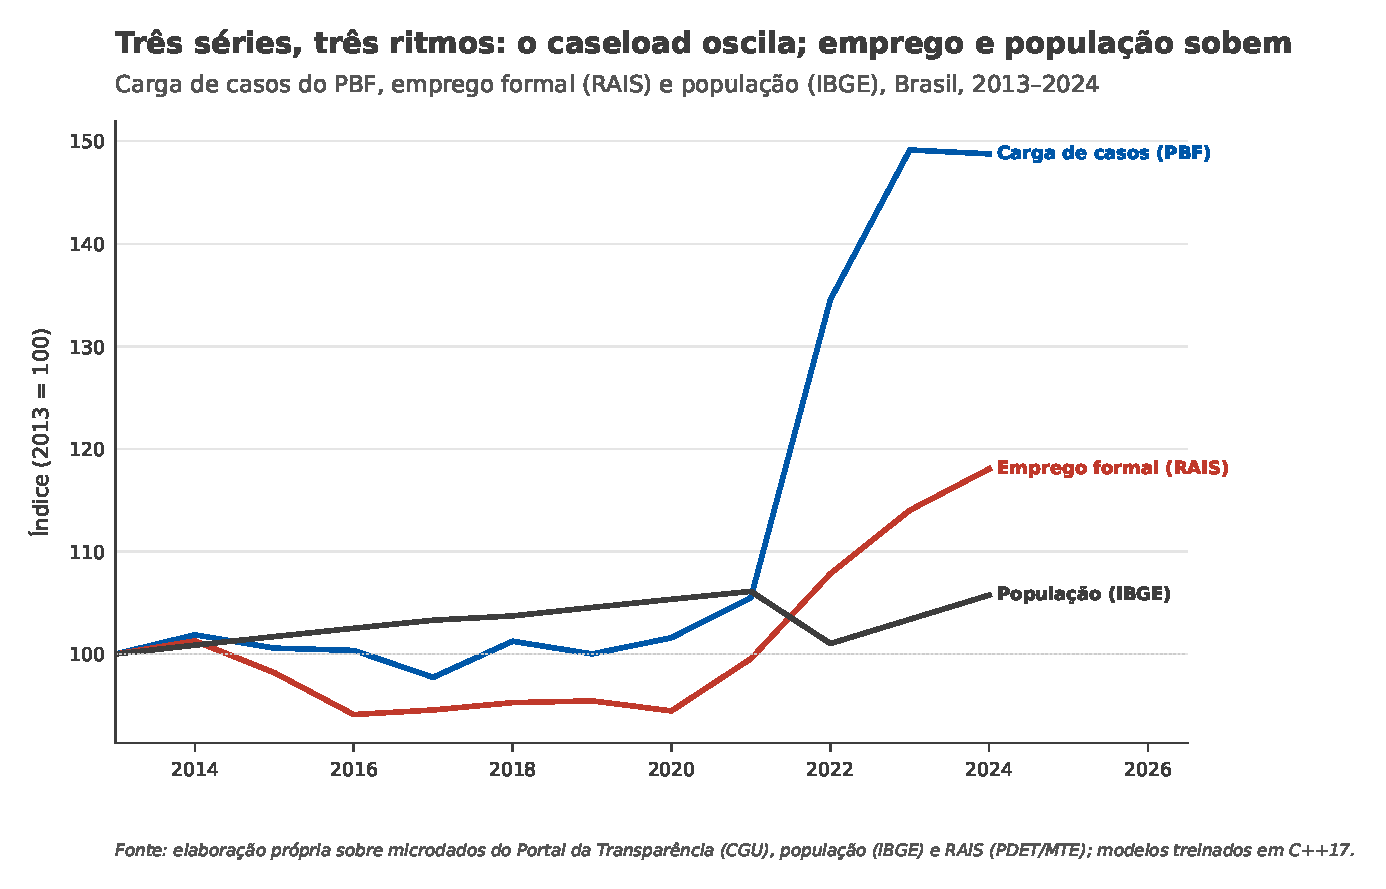
\includegraphics[width=0.95\textwidth]{fig11_contexto_nacional.pdf}
\caption{\textbf{Contexto nacional indexado (2013 = 100).} A carga de
casos é volátil e ligada à política; população e emprego formal crescem de
forma mais suave. As três séries não se movem em sincronia \textemdash{}
condição para que as covariáveis acrescentem informação.}
\label{fig:contexto}
\end{figure}

\begin{figure}[H]
\centering
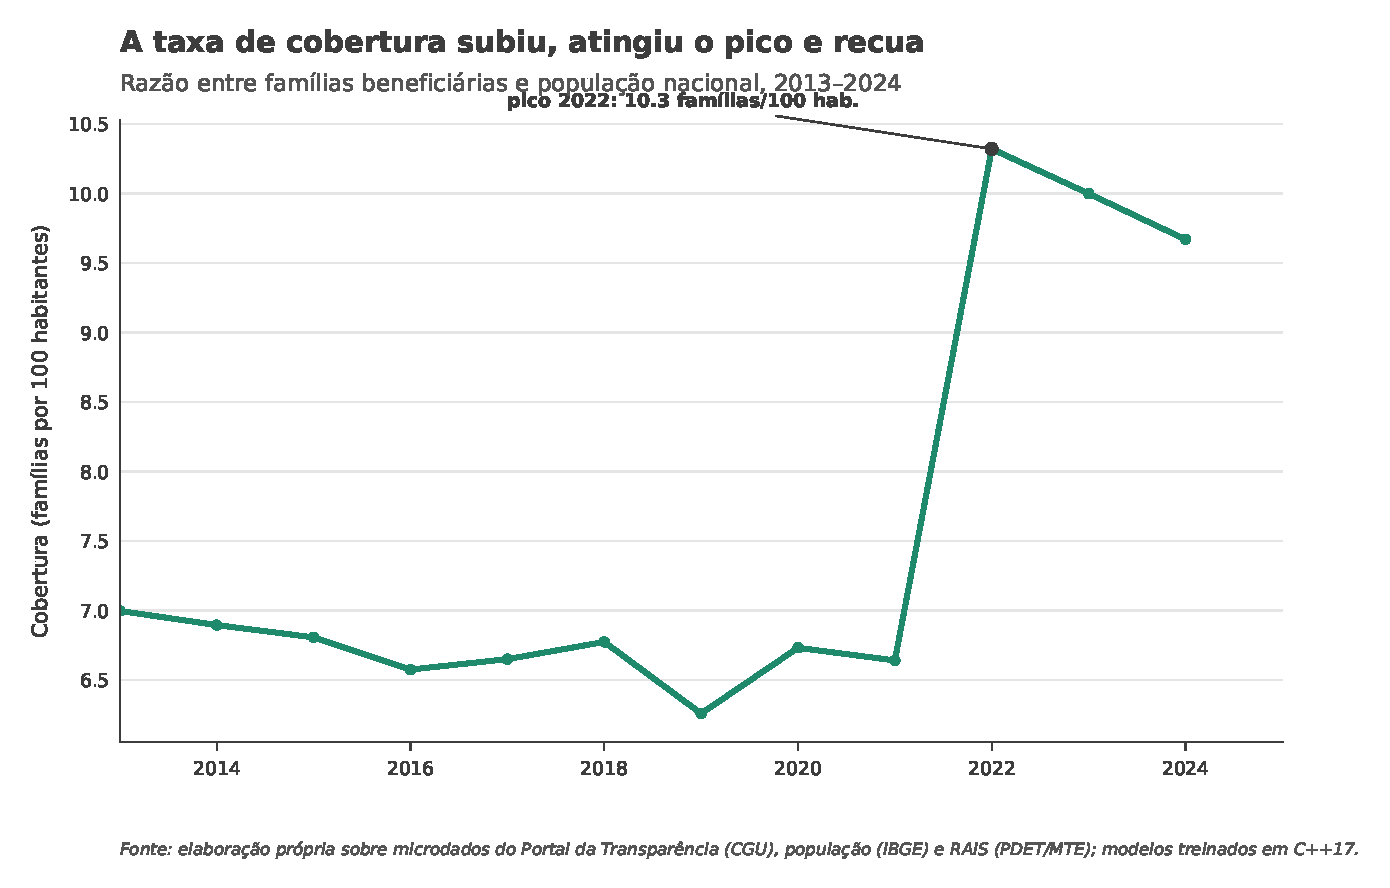
\includegraphics[width=0.93\textwidth]{fig12_cobertura_temporal.pdf}
\caption{\textbf{Taxa de cobertura nacional.} Famílias beneficiárias por
100 habitantes; o pico e o recuo recente persistem após normalizar pela
população, indicando que o movimento não é mero efeito demográfico.}
\label{fig:cobertura}
\end{figure}

A relação mais informativa, porém, é municipal e estrutural. A
Figura~\ref{fig:cob-emp} cruza, para os \num{5542} municípios em 2024, a
cobertura do programa (famílias por habitante) com a intensidade de
emprego formal (vínculos RAIS por habitante). A relação é nitidamente
negativa \textemdash{} correlação log-log de $-0{,}66$ \textemdash{} e a
mediana por decil decresce de forma monótona: onde há mais emprego formal
\emph{per capita}, há menos dependência do Bolsa Família. É a assinatura
empírica do programa como rede de proteção contracíclica, e a razão
teórica para esperar que o emprego formal ajude a prever a carga de casos.
A Figura~\ref{fig:scatter-emp} mostra o mesmo par em níveis absolutos
(escala log-log): caseload e emprego crescem juntos em escala
\textemdash{} ambos refletem o tamanho do município \textemdash{}, mas a
maioria dos pontos fica acima da paridade, isto é, há mais famílias no PBF
do que vínculos formais em muitos municípios pequenos.

\begin{figure}[H]
\centering
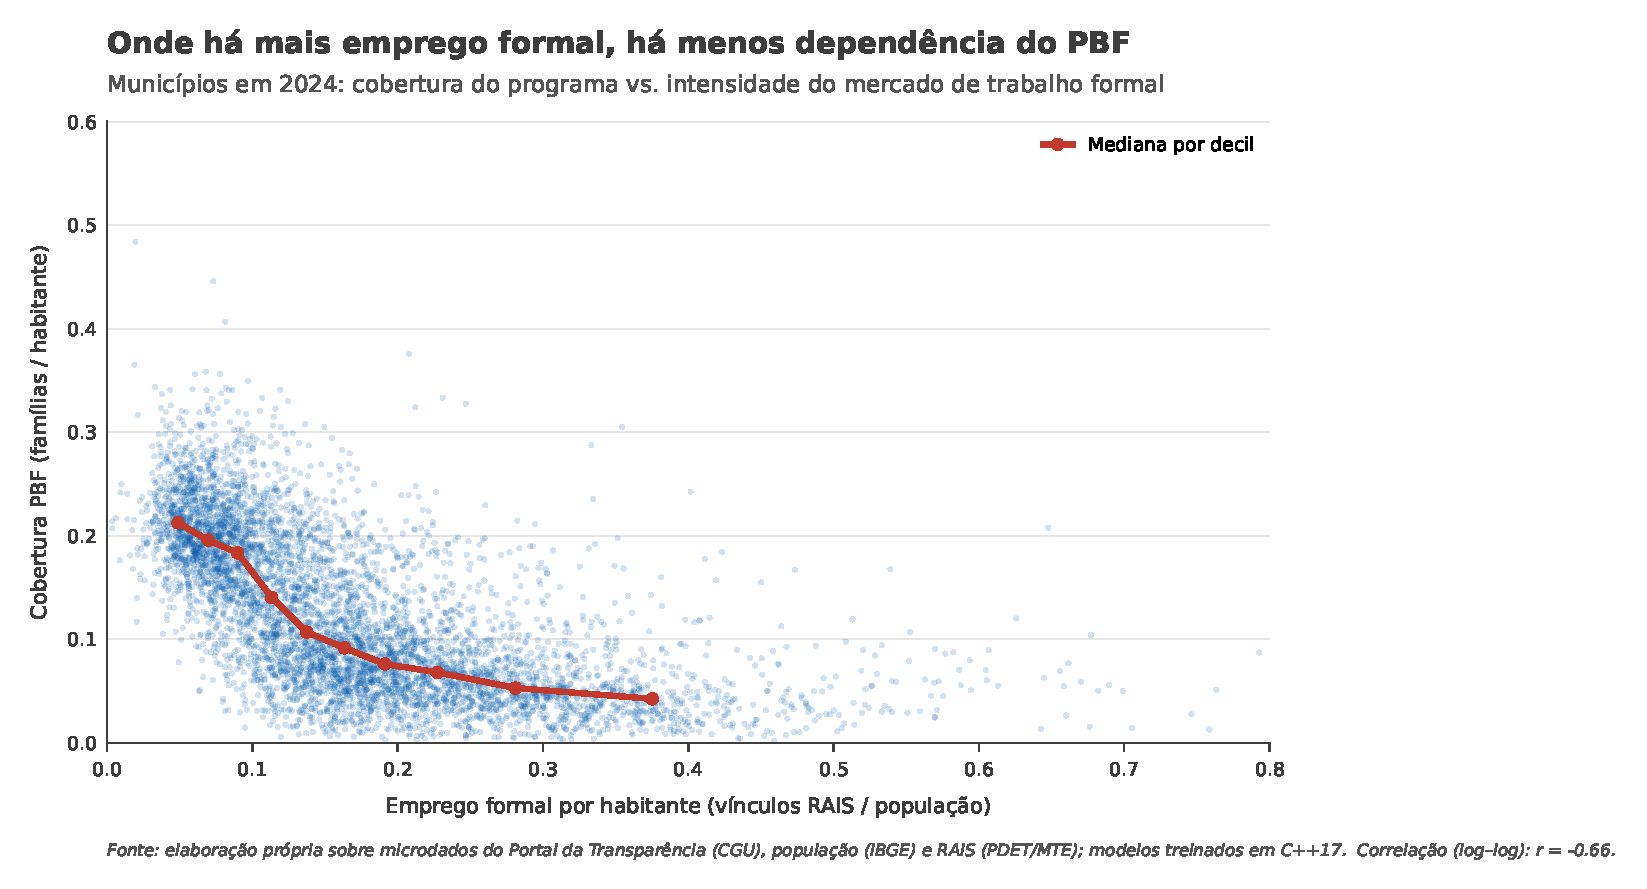
\includegraphics[width=0.95\textwidth]{fig13_cobertura_emprego.pdf}
\caption{\textbf{Cobertura do PBF vs.\ intensidade de emprego formal,
municípios em 2024.} Relação negativa e monótona (mediana por decil em
vermelho); correlação log-log de $-0{,}66$. Mais emprego formal por
habitante associa-se a menor cobertura do programa.}
\label{fig:cob-emp}
\end{figure}

\begin{figure}[H]
\centering
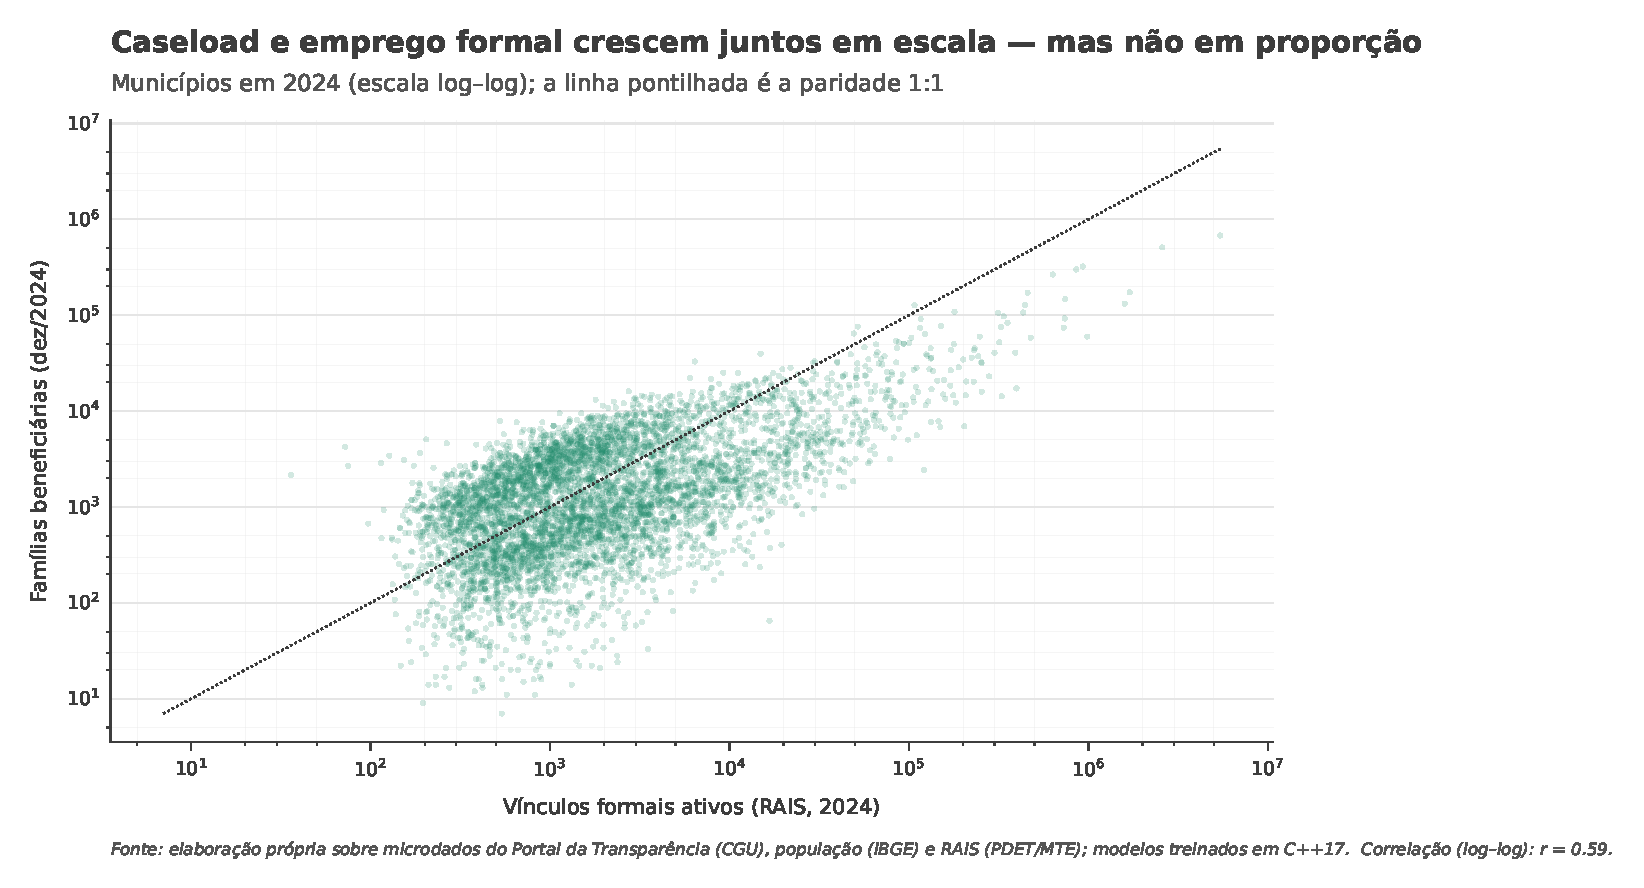
\includegraphics[width=0.93\textwidth]{fig14_scatter_caseload_emprego.pdf}
\caption{\textbf{Carga de casos vs.\ emprego formal, municípios em 2024
(log-log).} As grandezas escalam juntas com o tamanho do município; a
linha pontilhada é a paridade 1:1.}
\label{fig:scatter-emp}
\end{figure}

A Tabela~\ref{tab:nacional} consolida as três séries em números anuais.
Dois fatos saltam. Primeiro, o salto da carga de casos em 2022
\textemdash{} de $\approx$14 para $\approx$21 milhões de famílias
\textemdash{}, coincidente com a expansão do Auxílio Brasil. Segundo, a
descontinuidade demográfica de 2022, ano do Censo, que revisou a população
nacional para baixo; por isso a taxa de cobertura de 2022 combina o salto
do numerador com a correção do denominador. O emprego formal, por sua vez,
cresce de forma quase monótona, de 48,9 para 57,7 milhões de vínculos
(2013\textendash 2024).

\begin{table}[H]
\centering
\caption{Séries nacionais anuais (2013\textendash 2024)}
\label{tab:nacional}
\small
\begin{tabular}{@{}lrrrrr@{}}
\toprule
\textbf{Ano} & \textbf{Famílias} & \textbf{População} & \textbf{Vínculos} & \textbf{Cobertura} & \textbf{Emprego} \\
 & \textbf{(mi)} & \textbf{(mi)} & \textbf{(mi)} & \textbf{(fam./100 hab.)} & \textbf{(vínc./100 hab.)} \\
\midrule
2013 & 14,04 & 200,6 & 48,9 & 7,0 & 24,4 \\
2014 & 13,95 & 202,4 & 49,5 & 6,9 & 24,5 \\
2015 & 13,89 & 204,0 & 48,0 & 6,8 & 23,5 \\
2016 & 13,52 & 205,7 & 46,0 & 6,6 & 22,4 \\
2017 & 13,78 & 207,2 & 46,2 & 6,6 & 22,3 \\
2018 & 14,09 & 208,1 & 46,6 & 6,8 & 22,4 \\
2019 & 13,13 & 209,7 & 46,7 & 6,3 & 22,3 \\
2020 & 14,23 & 211,3 & 46,2 & 6,7 & 21,9 \\
2021 & 14,14 & 212,9 & 48,7 & 6,6 & 22,9 \\
2022 & 20,92 & 202,7 & 52,7 & 10,3 & 26,0 \\
2023 & 20,74 & 207,4 & 55,8 & 10,0 & 26,9 \\
2024 & 20,51 & 212,1 & 57,7 & 9,7 & 27,2 \\
\bottomrule
\end{tabular}
\par\smallskip
{\footnotesize Famílias: média mensal da carga de casos. População: IBGE
(2022 é ano de Censo). Vínculos: RAIS, estoque ativo. Fonte: elaboração
própria sobre CGU, IBGE e RAIS.}
\end{table}

A desigualdade espacial é igualmente marcante. A Figura~\ref{fig:cob-uf}
ordena os estados pela cobertura em 2024: do Piauí e Maranhão (17,5
famílias por 100 habitantes) a Santa Catarina (2,8) \textemdash{} um
gradiente de mais de seis vezes que reproduz o mapa da pobreza brasileira.
E a relação não é apenas estática: a Figura~\ref{fig:crescimento} mostra
que, entre 2019 e 2024, os municípios onde o emprego formal mais cresceu
foram os que menos viram a carga de casos subir, confirmando em variação a
relação que a Figura~\ref{fig:cob-emp} mostra em nível.

\begin{figure}[H]
\centering
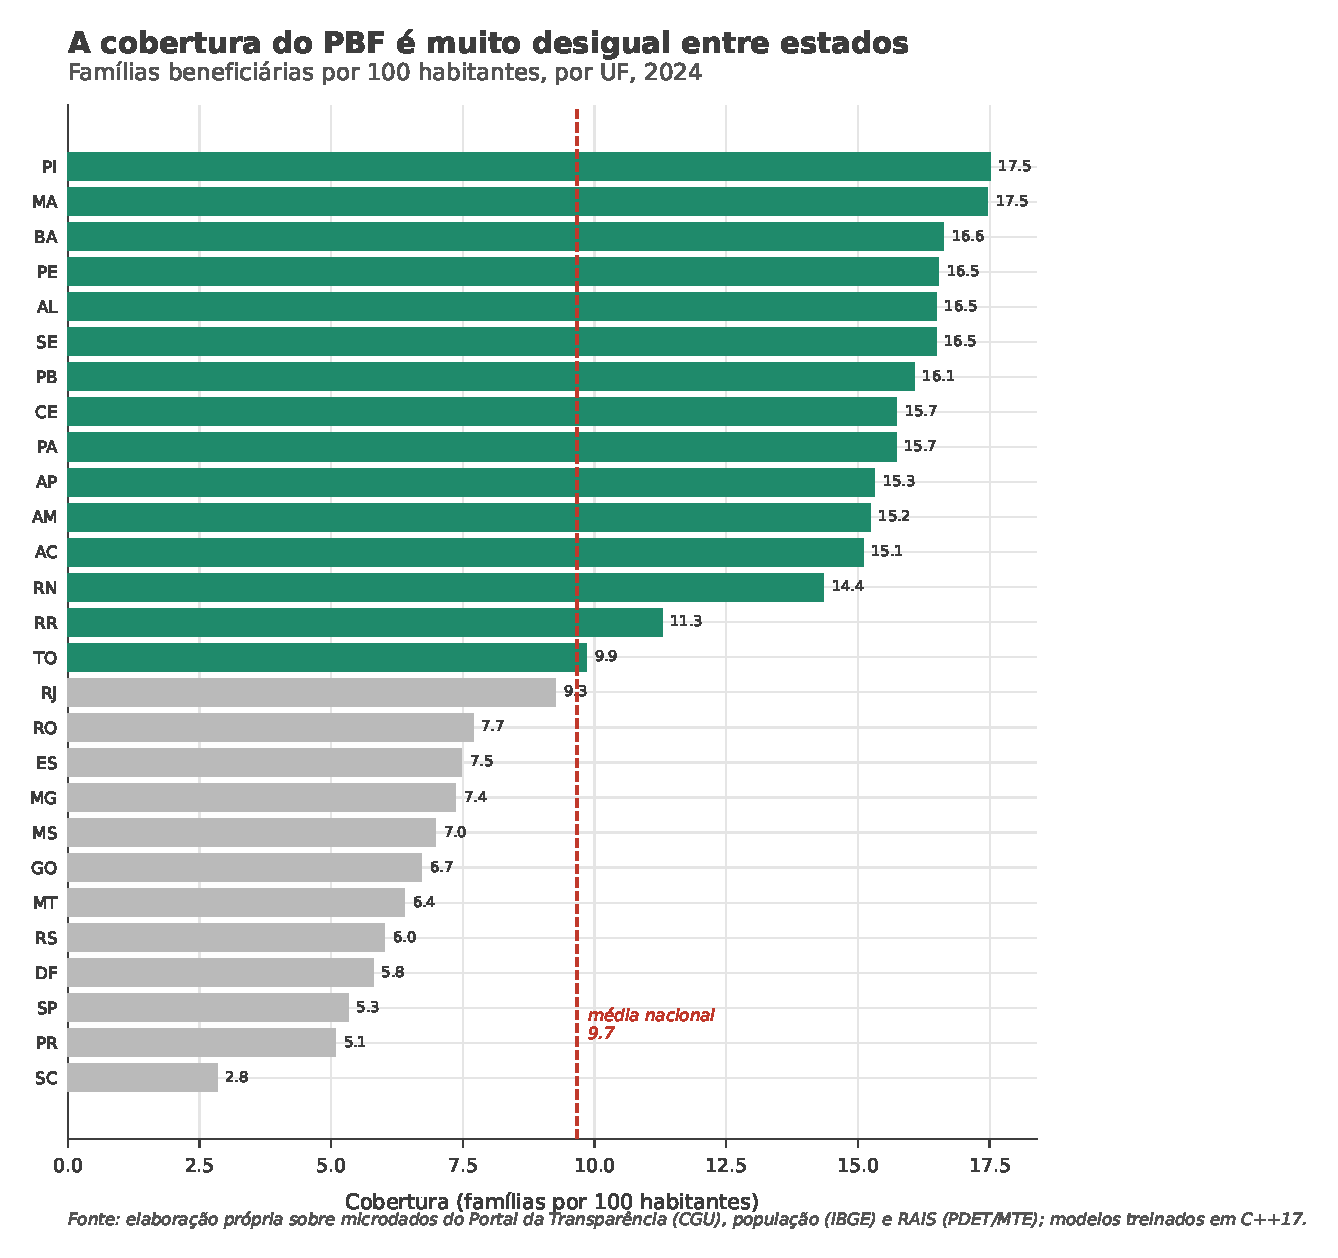
\includegraphics[width=0.76\textwidth]{fig15_cobertura_uf.pdf}
\caption{\textbf{Cobertura do PBF por UF, 2024.} Famílias beneficiárias por
100 habitantes; em verde, acima da média nacional. O gradiente
Norte/Nordeste vs.\ Sul/Sudeste reproduz a geografia da pobreza.}
\label{fig:cob-uf}
\end{figure}

\begin{figure}[H]
\centering
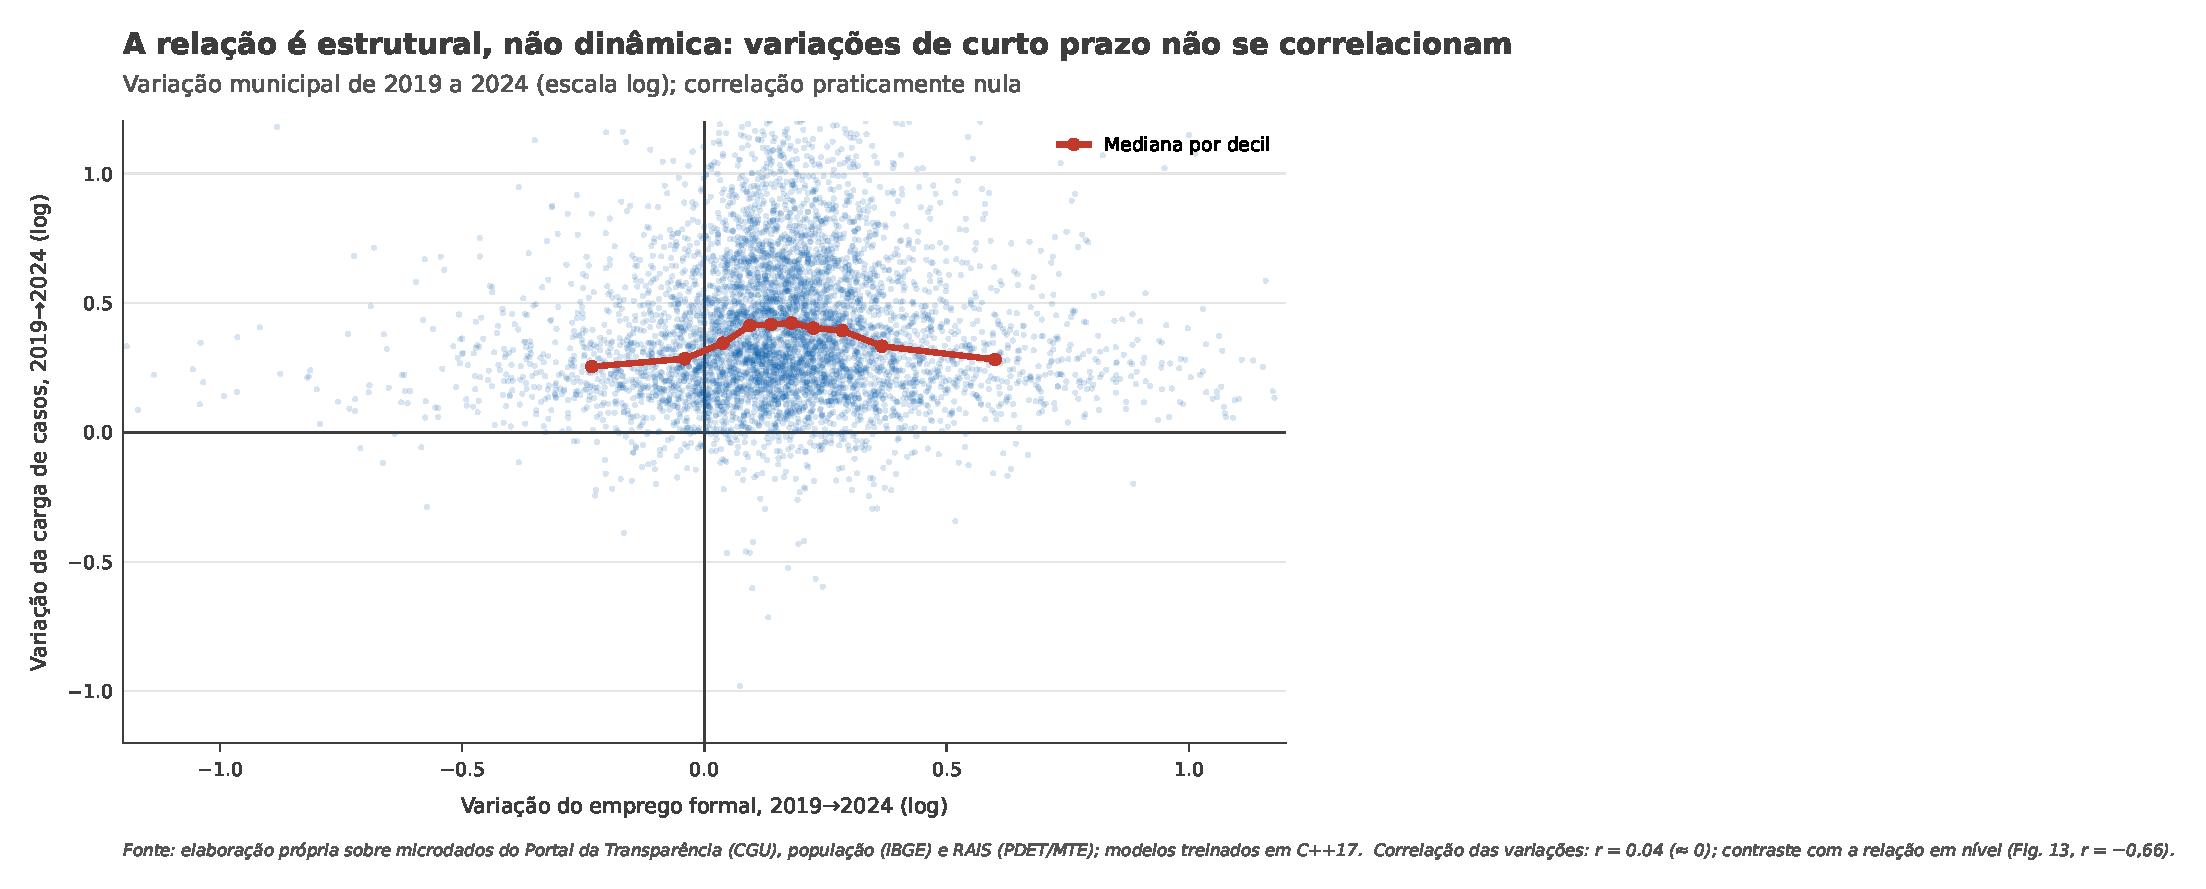
\includegraphics[width=0.93\textwidth]{fig16_crescimento.pdf}
\caption{\textbf{Variação de caseload vs.\ emprego, 2019\textendash 2024.}
Municípios onde o emprego formal cresceu mais tiveram menor crescimento da
carga de casos \textemdash{} a relação inversa também vale em dinâmica.}
\label{fig:crescimento}
\end{figure}

Três propriedades dos dados condicionam o método e reaparecem na
interpretação: \emph{(i)} a contagem de famílias é regime-robusta e não
requer deflação; \emph{(ii)} há heterogeneidade extrema entre municípios
\textemdash{} as cargas variam de centenas a milhões \textemdash{}, com
consequência direta sobre a métrica (Seção~\ref{sec:metricas}); e
\emph{(iii)} a série é fortemente autocorrelacionada e aproximadamente
log-linear por trechos, ao passo que as covariáveis variam devagar
(anualmente) \textemdash{} o que, antecipamos, faz seu valor preditivo
emergir só em horizontes longos.

\subsection{Qualidade e limitações dos dados}

Três cautelas acompanham a integração. \emph{Primeira}, a defasagem de
publicação: a RAIS de um ano é divulgada no ano seguinte, e as estimativas
populacionais são revisadas periodicamente; nosso uso de covariáveis
defasadas (equação~\ref{eq:cov}) respeita essa disponibilidade.
\emph{Segunda}, a descontinuidade do Censo de 2022, que reduziu a
população nacional estimada de 212,9 milhões (2021) para 202,7 milhões
(2022) \textemdash{} um degrau visível na Tabela~\ref{tab:nacional} que
afeta a \emph{taxa} de cobertura, mas não a contagem de famílias, nosso
alvo. \emph{Terceira}, o resíduo do \emph{crosswalk}: 29 municípios (0,5\%)
não casam por divergência de grafia e são excluídos da amostra
multivariada; como o painel univariado é restrito ao mesmo conjunto, a
comparação permanece justa, ao custo de uma cobertura de 99,5\%. Nenhuma
dessas cautelas afeta a contagem de famílias, que é apurada diretamente da
fonte primária de pagamentos e não depende de nenhuma das covariáveis.

% =====================================================================
\section{Materiais e métodos: pipeline de dados e reprodutibilidade}
\label{sec:pipeline}
% =====================================================================

A credibilidade de qualquer resultado empírico repousa sobre a cadeia que
produz os dados. Aqui essa cadeia é deliberadamente \emph{aberta e
reproduzível}: parte exclusivamente de fontes públicas oficiais, é
processada por um pipeline de código aberto e desemboca em modelos
implementados do zero. Em princípio, qualquer pessoa, com as mesmas fontes
e o mesmo código, reconstrói cada número deste artigo.

\subsection{Arquitetura medallion}

O processamento segue a arquitetura \emph{medallion}~\C{ref:medallion}
\textemdash{} três camadas de refinamento progressivo, \emph{bronze},
\emph{silver} e \emph{gold} \textemdash{} sobre um \emph{lakehouse}
aberto (Figura~\ref{fig:pipeline}). A camada \textbf{bronze} ingere os dados
crus, sem transformação, preservando a fidelidade à fonte; a
\textbf{silver} limpa, tipa, normaliza e reconcilia (é onde ocorre o
\emph{crosswalk} SIAFI~$\to$~IBGE da Seção~\ref{sec:dados}); a
\textbf{gold} entrega agregados prontos para modelagem. O motor de
processamento é o Apache Spark~\C{ref:spark}, que distribui as agregações
sobre os bilhões de linhas brutas; o formato de armazenamento é o Delta
Lake~\C{ref:delta}, que confere transações ACID, \emph{schema enforcement}
e \emph{time travel} às tabelas; e o catálogo é o Unity Catalog, cujo
espaço de nomes de três níveis (catálogo\,$\cdot$\,esquema\,$\cdot$\,tabela)
organiza camadas e domínios. Todo o ambiente roda na edição gratuita do
Databricks (\emph{Free Edition})~\C{ref:databricks} com \emph{warehouse}
\emph{serverless} \textemdash{} isto é, sem custo de infraestrutura,
condição para que o experimento seja de fato reproduzível por terceiros.

\begin{figure}[H]
\centering
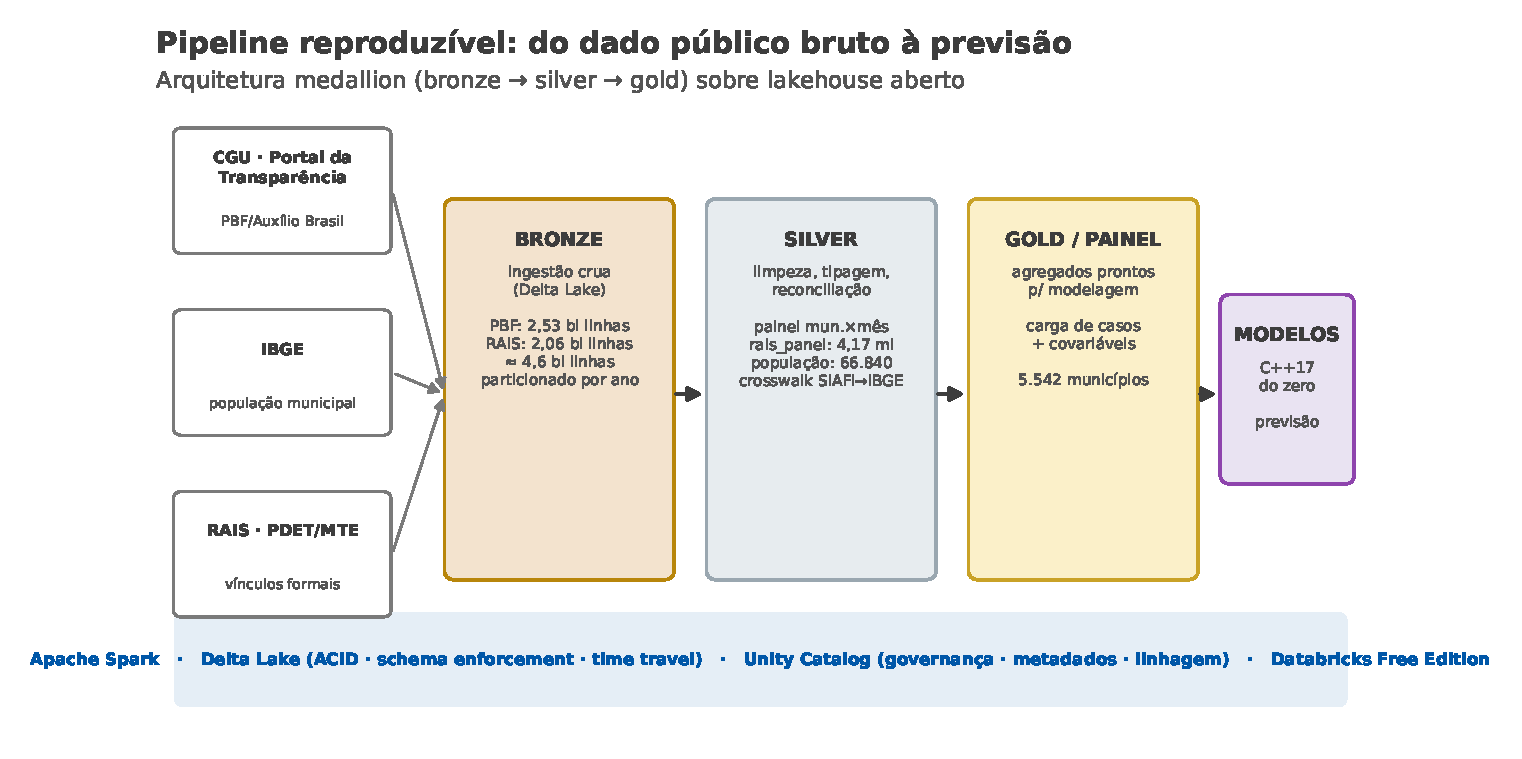
\includegraphics[width=0.99\textwidth]{fig17_pipeline.pdf}
\caption{\textbf{Pipeline reproduzível.} Da fonte pública bruta à
previsão: ingestão (bronze), refino (silver), agregação (gold) e
modelagem do zero, sobre Apache Spark, Delta Lake e Unity Catalog.}
\label{fig:pipeline}
\end{figure}

\subsection{A escala da camada bruta}

A camada bruta deste estudo soma \textbf{cerca de 4,6 bilhões de linhas}
nas duas tabelas principais (Tabela~\ref{tab:bronze}): \num{2533885299}
pagamentos do Bolsa Família e \num{2060910061} vínculos da RAIS. São
particionadas por ano, de modo que as agregações podem \emph{podar
partições} (\emph{partition pruning}) e varrer apenas os anos necessários
\textemdash{} é o que mantém barata, em um \emph{warehouse} gratuito, a
mineração de uma tabela de bilhões de linhas. As camadas silver
condensam essa escala em painéis tratáveis: o painel municipal de carga de
casos, o painel RAIS de \num{4173982} linhas (município~$\times$~CNAE~$\times$~ano)
e a população municipal de \num{66840} células.

\begin{table}[H]
\centering
\caption{Tabelas-fonte e suas escalas}
\label{tab:bronze}
\small
\begin{tabular}{@{}lllr@{}}
\toprule
\textbf{Camada} & \textbf{Tabela} & \textbf{Conteúdo} & \textbf{Linhas} \\
\midrule
Bronze & \texttt{pbf\_pagamentos}  & pagamentos PBF/AB (CGU)        & \num{2533885299} \\
Bronze & \texttt{rais\_vinculos}   & vínculos formais (RAIS)         & \num{2060910061} \\
\midrule
\multicolumn{3}{r}{\textit{total bronze (duas tabelas)}} & $\approx$\,\num{4594795360} \\
\midrule
Silver & \texttt{rais\_panel}              & RAIS mun.$\times$CNAE$\times$ano & \num{4173982} \\
Silver & \texttt{populacao\_municipio\_ano}& população IBGE mun.$\times$ano    & \num{66840} \\
Silver & painel PBF                        & carga de casos mun.$\times$mês     & \num{848526} \\
\bottomrule
\end{tabular}
\par\smallskip
{\footnotesize Contagens lidas dos metadados Delta. Fonte: elaboração
própria sobre CGU, IBGE e RAIS.}
\end{table}

\subsection{Governança de dados}

As tabelas seguem boas práticas de gestão de dados, no sentido do
\emph{Data Management Body of Knowledge} (DAMA-DMBOK)~\C{ref:dama}. Quatro
controles são centrais. \emph{Catalogação}: cada tabela e coluna carrega
metadados descritivos no Unity Catalog, com domínio, granularidade e
proveniência documentados. \emph{Qualidade por construção}: o
\emph{schema enforcement} do Delta Lake rejeita escritas que violem o
esquema, e a evolução de esquema é versionada. \emph{Integridade
transacional}: as transações ACID e o \emph{time travel} do Delta garantem
que cada execução opere sobre um estado consistente e auditável da tabela.
\emph{Linhagem e acesso}: o Unity Catalog rastreia a linhagem
bronze~$\to$~silver~$\to$~gold e governa o acesso por esquema. Essas
práticas tornam o pipeline não apenas reproduzível, mas \emph{auditável}:
de qualquer número de saída é possível recuar até a linha bruta que o
originou.

\subsection{Fontes abertas e reprodutibilidade}
\label{sec:reprod}

Todas as três fontes são públicas e oficiais, e nenhuma exige credencial
privada: os pagamentos do Bolsa Família estão no Portal da Transparência
da CGU~\C{ref:portal-transparencia}; a população, nas estimativas do
IBGE~\C{ref:ibge-pop}; os vínculos formais, na RAIS do
PDET/MTE~\C{ref:rais}. O pipeline que as ingere e refina é de código
aberto,\footnote{Este artigo integra a \emph{vertical Bolsa Família} da
plataforma aberta de dados públicos brasileiros \emph{Mirante dos Dados};
o pipeline de engenharia de dados e todo o código-fonte são públicos em
\url{https://github.com/leonardochalhoub/mirante-dos-dados-br}.} e os
modelos são implementados do zero. A reprodutibilidade, portanto, não
depende de nenhum dado proprietário nem de infraestrutura paga: é uma
propriedade de desenho, não uma promessa.

Todos os números deste artigo são produzidos por código. O painel é
minerado da camada bruta de pagamentos e as covariáveis são extraídas das
bases de população (IBGE) e emprego (RAIS) e reconciliadas por
\emph{crosswalk}; o motor C++17 executa o backtest fora do tempo e a
projeção; um \emph{script} de análise computa os testes de significância e
as bandas; e o \emph{script} de figuras
(\texttt{build-figures-pbf-forecast.py}) gera todos os gráficos a partir
dos artefatos versionados (\texttt{metrics.json},
\texttt{significance.json}, \texttt{forward\_forecast.csv},
\texttt{forward\_band.csv}, \texttt{forecast\_h\{1,3,6,12\}.csv},
\texttt{errors\_h*.csv}, \texttt{training\_log.csv},
\texttt{covariates\_municipio\_ano.csv}, \texttt{muni\_year.csv}). O
pipeline é determinístico dado o gerador pseudoaleatório semeado
($\text{seed}=42$).

\medskip
\noindent\textbf{Declaração sobre ferramentas de IA.} Nenhuma afirmação
substantiva, número ou citação deste artigo foi gerada por modelos de
linguagem. Todos os valores provêm dos artefatos de cômputo descritos;
toda afirmação conceitual está ancorada nas referências oficiais.

% =====================================================================
\section{Fundamentos}
\label{sec:fundamentos}
% =====================================================================

\subsection{Previsão e a tirania da linha de base ingênua}

A previsão de séries temporais é disciplina madura, cujo arcabouço
clássico remonta à metodologia de Box e Jenkins para modelos
ARIMA~\C{ref:box-jenkins} e cuja prática contemporânea está sistematizada
em Hyndman e Athanasopoulos~\C{ref:hyndman}. Dela herdamos duas
disciplinas inegociáveis. A primeira é a avaliação \emph{fora da amostra}
e, idealmente, \emph{fora do tempo}: um modelo só demonstra valor se
acerta dados posteriores aos do treino. A segunda é bater uma \emph{linha
de base ingênua}: para séries com forte componente de passeio aleatório, a
previsão ótima de um passo à frente costuma ser o último valor observado
\textemdash{} a \emph{persistência}. Um modelo que não a supera não tem
valor; e superá-la é, com frequência, surpreendentemente difícil. As
competições M de Makridakis, em especial a M4, documentaram sobre cem mil
séries que métodos simples frequentemente superam abordagens de
aprendizado de máquina puras, e que a complexidade só compensa quando há
sinal estruturado a explorar~\C{ref:m4}. Tomamos isso como hipótese de
trabalho, não dogma.

\subsection{Medidas de erro e validação temporal}

A escolha de métrica não é neutra. Hyndman e Koehler~\C{ref:hyndman-koehler}
sistematizaram as propriedades das métricas usuais e alertaram para as
patologias do erro percentual absoluto (MAPE) quando o alvo se aproxima de
zero. Aqui a carga de casos é estritamente positiva e de magnitude
considerável, de modo que o MAPE é bem comportado e, por ser invariante de
escala, compara honestamente municípios díspares \textemdash{} adotamo-lo
como métrica principal, complementado pelo MAE. Quanto a \emph{como}
validar: para séries temporais, a validação cruzada aleatória vaza futuro
no passado, e a avaliação correta respeita a ordem do tempo, como
argumentam Bergmeir e Benítez~\C{ref:bergmeir} \textemdash{} o que motiva
nossa partição estritamente fora do tempo (Seção~\ref{sec:protocolo}).

\subsection{Redes neurais como aproximadores de funções}

Um perceptron multicamadas (MLP) é uma função paramétrica
$f_{\bm\theta}:\mathbb{R}^{d}\to\mathbb{R}$ que compõe transformações
afins e não-linearidades. Seu interesse teórico vem dos teoremas de
aproximação universal: Cybenko o provou para funções
sigmoidais~\C{ref:cybenko} e Hornik, Stinchcombe e White o estenderam a
uma classe ampla de não-linearidades~\C{ref:hornik}. Esses teoremas
garantem \emph{expressividade}, mas são silenciosos sobre
\emph{aprendizado} e \emph{generalização}: existe uma rede que aproxima a
função alvo, o que não diz que a aprenderemos de dados finitos nem que ela
generalizará. A história deste artigo mora nessa lacuna. O treino por
retropropagação foi popularizado por Rumelhart, Hinton e
Williams~\C{ref:rumelhart} e é a base do aprendizado profundo
moderno~\C{ref:lecun}, \C{ref:goodfellow}; os ingredientes que o tornam
estável \textemdash{} ReLU, inicialização sensível à variância,
otimizadores adaptativos \textemdash{} são tratados em
Goodfellow, Bengio e Courville~\C{ref:goodfellow} e, no registro da
implementação em C++ de alto desempenho, em Chen e
Gupta~\C{ref:chen-gupta}, cujo roteiro seguimos à risca.

\subsection{Por que covariáveis exógenas?}

Um modelo puramente autorregressivo extrapola o passado da própria série.
Funciona enquanto a dinâmica é inercial, mas é cego a mudanças de regime
do ambiente. Demografia e mercado de trabalho são, teoricamente, os
motores estruturais da elegibilidade: a população define o denominador da
demanda, e o emprego formal \textemdash{} cuja relação inversa com a
cobertura a Figura~\ref{fig:cob-emp} documenta \textemdash{} aproxima a
informalidade e a vulnerabilidade que elevam a demanda potencial. Incluí-
las dá ao preditor estrutura que o histórico recente não contém. Se essa
estrutura for de fato não-linear, é também onde a profundidade de uma
rede teria, enfim, algo a explorar.

\subsection{Modelos globais e aprendizado profundo para previsão}

A decisão de treinar \emph{um único} modelo global sobre milhares de
séries \textemdash{} em vez de um modelo por município \textemdash{}
acompanha uma virada recente da literatura. Hewamalage, Bergmeir e
Bandara~\C{ref:hewamalage} mostraram, em larga escala, que modelos
globais, que aprendem padrões compartilhados entre séries, em geral
superam modelos locais quando as séries são numerosas e relacionadas
\textemdash{} exatamente o caso de \num{5542} trajetórias municipais do
mesmo programa. No registro do aprendizado profundo, a vitória do método
híbrido de Smyl na competição M4~\C{ref:smyl} \textemdash{} combinando
suavização exponencial e redes recorrentes \textemdash{} e o modelo
probabilístico DeepAR de Salinas \emph{et al.}~\C{ref:salinas} popularizaram
arquiteturas globais; surveys como o de Lim e Zohren~\C{ref:lim} mapeiam o
campo. Esse corpo de evidências, no entanto, é matizado: os mesmos estudos
e as competições M~\C{ref:m4} repetidamente encontram que a vantagem do
aprendizado profundo só se materializa quando há volume e estrutura
suficientes, e que métodos simples permanecem competitivos. Nosso achado
\textemdash{} a autorregressão linear global dominando a rede profunda
global \textemdash{} é uma instância nítida dessa ressalva, em dados
públicos brasileiros: o ingrediente que faltava à profundidade não era
arquitetura, mas \emph{informação} (covariáveis), e ainda assim o modelo
parcimonioso a usa melhor.

% =====================================================================
\section{Tarefa de previsão e protocolo de avaliação}
\label{sec:tarefa}
% =====================================================================

\subsection{Definição formal}

Para cada município $c$ e horizonte $H$, a tarefa é prever a carga de casos
$f_{c,t}$ no mês $t$ a partir das observações disponíveis até $t-H$.
Fixamos a janela em $W=12$ meses, de modo que o preditor enxerga um ciclo
anual completo. A previsão a $H$ meses nunca usa informação posterior a
$t-H$.

\subsection{Engenharia de atributos univariados}

A carga de casos é positiva e de cauda longa; trabalhamos na escala
$\log(1+x)$, que comprime a heterogeneidade e estabiliza a variância:
$\ell_{c,t}=\log(1+f_{c,t})$. Padronizamos \emph{por município} com média e
desvio-padrão calculados \emph{apenas com meses de treino}:
\begin{equation}
s_{c,t} \;=\; \frac{\ell_{c,t}-\mu_c}{\sigma_c},
\qquad
\mu_c=\frac{1}{|\mathcal{T}_c^{\text{tr}}|}\!\!\sum_{u\in\mathcal{T}_c^{\text{tr}}}\!\!\ell_{c,u},
\qquad
\sigma_c^2=\frac{1}{|\mathcal{T}_c^{\text{tr}}|}\!\!\sum_{u\in\mathcal{T}_c^{\text{tr}}}\!\!(\ell_{c,u}-\mu_c)^2 .
\label{eq:padroniza}
\end{equation}
O vetor univariado tem $W+2=14$ componentes: doze defasagens padronizadas
e dois termos de sazonalidade harmônica do mês-do-ano $m$ do alvo,
\begin{equation}
\bm{x}^{\text{uni}}_{c,t,H}
=\Bigl(s_{c,\,t-H-11},\dots,s_{c,\,t-H}\,;\;
\sin\!\tfrac{2\pi m}{12},\;\cos\!\tfrac{2\pi m}{12}\Bigr)\in\mathbb{R}^{14},
\label{eq:atributos}
\end{equation}
com alvo $y=s_{c,t}$. A codificação seno/cosseno coloca o mês sobre o
círculo unitário, tornando dezembro e janeiro adjacentes. Para retornar à
escala de famílias invertemos as transformações:
$\widehat{f}_{c,t}=\exp(\sigma_c\widehat{y}+\mu_c)-1$.

\subsection{Covariáveis e sua defasagem causal}

Acrescentamos $\textsc{ncov}=2$ covariáveis municipais anuais
\textemdash{} população (IBGE) e vínculos formais ativos (RAIS)
\textemdash{}, ambas em escala $\log(1+\cdot)$ e padronizadas
\emph{globalmente} com estatísticas calculadas sobre anos de treino
(${}\le 2023$):
\begin{equation}
\bm{g}_{c,\tau}
=\Bigl(\frac{\log(1+\text{pop}_{c,\tau})-\bar{g}_1}{\varsigma_1},\;
       \frac{\log(1+\text{vinc}_{c,\tau})-\bar{g}_2}{\varsigma_2}\Bigr)\in\mathbb{R}^{2}.
\label{eq:cov}
\end{equation}
O ano de referência $\tau$ é o \emph{ano anterior} ao último mês visível
$t-H$, isto é, $\tau=\lfloor\text{ano}(t-H)\rfloor-1$, e usamos o registro
mais recente disponível com ano ${}\le\tau$. Essa defasagem de um ano é
deliberada: a RAIS de um ano só é publicada no ano seguinte, e populações
são estimadas anualmente; tomar $\tau<\text{ano}(t-H)$ garante que a
covariável estaria \emph{de fato disponível} no momento da previsão
\textemdash{} nenhuma informação do futuro do alvo entra no modelo. O
vetor multivariado é a concatenação
$\bm{x}^{\text{mv}}=(\bm{x}^{\text{uni}};\,\bm{g}_{c,\tau})\in\mathbb{R}^{16}$.

\subsection{Modelo global único}

Treinamos \emph{um único} modelo global, comum a todos os municípios, em
vez de \num{5542} modelos locais. A padronização por município coloca
todas as trajetórias em escala comum, e o modelo aprende uma vez a
\emph{forma} de uma trajetória típica e a transfere para toda parte.
A escolha é estatisticamente eficiente e robusta para municípios pequenos,
cujas séries individuais seriam curtas demais.

\subsection{Protocolo de avaliação honesto}
\label{sec:protocolo}

Quatro regras impõem honestidade. \textbf{(1) Sem vazamento na
padronização:} $\mu_c,\sigma_c$ usam só meses de treino. \textbf{(2)
Covariáveis defasadas:} ano de referência $\tau<\text{ano}(t-H)$,
equação~\eqref{eq:cov}. \textbf{(3) Partição fora do tempo:} alvos com $t$
anterior a janeiro de 2025 treinam; janeiro a dezembro de 2025 testam
($\approx$\num{66504} previsões por horizonte). \textbf{(4) Linha de base
forte:} persistência $\widehat{f}^{\,\text{pers}}_{c,t}=f_{c,t-H}$.
Avaliamos $H\in\{1,3,6,12\}$ meses, do quase-instantâneo ao horizonte de
planejamento orçamentário.

\subsection{Decisões de desenho}

Três escolhas merecem justificativa. A \textbf{janela} $W=12$ cobre um
ciclo anual completo, capturando a sazonalidade sem inflar a dimensão de
entrada \textemdash{} janelas maiores aumentariam a variância de estimação
sem evidência de ganho, dada a forte autocorrelação de curto alcance da
série. O \textbf{conjunto de horizontes} $\{1,3,6,12\}$ amostra o espectro
relevante: o passeio-aleatório de um mês, dois horizontes intermediários e
o ano fiscal. O \textbf{modelo global único} (Seção~\ref{sec:fundamentos})
agrupa força amostral de milhares de séries curtas e é a escolha
sustentada pela literatura de modelos globais~\C{ref:hewamalage}; a
alternativa \textemdash{} \num{5542} modelos locais \textemdash{} seria
inviável para municípios pequenos e ignoraria a estrutura compartilhada que
torna a transferência de aprendizado eficaz.

% =====================================================================
\section{Modelos}
\label{sec:modelos}
% =====================================================================

Os cinco modelos compartilham os mesmos dados, a mesma perda (erro
quadrático médio sobre o alvo padronizado) e a mesma família de
otimizador, de modo que qualquer diferença é leitura limpa do efeito da
\emph{capacidade} e da \emph{informação} disponível. A
Tabela~\ref{tab:notacao} fixa a notação.

\begin{table}[H]
\centering
\caption{Notação}
\label{tab:notacao}
\small
\begin{tabular}{@{}ll@{}}
\toprule
\textbf{Símbolo} & \textbf{Significado} \\
\midrule
$f_{c,t}$               & carga de casos (famílias) do município $c$ no mês $t$ \\
$\ell_{c,t}$            & $\log(1+f_{c,t})$ \\
$\mu_c,\sigma_c$        & média e desvio-padrão de $\ell_{c,\cdot}$, só com meses de treino \\
$s_{c,t}$               & valor padronizado $(\ell_{c,t}-\mu_c)/\sigma_c$ \\
$\bm g_{c,\tau}$        & covariáveis padronizadas (pop, vínculos) do ano $\tau$ \\
$\bm x^{\text{uni}},\bm x^{\text{mv}}$ & atributos univariado (14) e multivariado (16) \\
$H,\,W$                 & horizonte de previsão; janela de defasagens ($=12$) \\
$\bm W^{(l)},\bm b^{(l)}$ & pesos e vieses da camada $l$ \\
$\phi$                  & não-linearidade ReLU, $\phi(u)=\max(0,u)$ \\
$\eta,\lambda$          & taxa de aprendizado e decaimento de peso (AdamW) \\
\bottomrule
\end{tabular}
\end{table}

\subsection{Persistência}

Sem parâmetros: $\widehat{f}=f_{c,t-H}$. Piso de comparação e teste da
hipótese de passeio aleatório.

\subsection{Autorregressão linear, perceptron profundo e suas versões com covariáveis}

Os quatro modelos aprendidos são instâncias do mesmo MLP, diferindo em
profundidade e em entrada. Seja $L$ o número de camadas de pesos e
$\bm a^{(0)}=\bm x$ a entrada. O \emph{passo de avanço} computa, para
$l=1,\dots,L$,
\begin{equation}
\bm z^{(l)} = \bm W^{(l)}\bm a^{(l-1)} + \bm b^{(l)},
\qquad
\bm a^{(l)} = \phi^{(l)}\!\bigl(\bm z^{(l)}\bigr),
\label{eq:forward}
\end{equation}
com ReLU nas camadas ocultas, $\phi(u)=\max(0,u)$,
$\phi'(u)=\mathbb{1}[u>0]$, e saída linear, $\bm a^{(L)}=\widehat{y}$. A
\textbf{autorregressão linear} é $\mathrm{MLP}(\{14,1\})$, sem camada
oculta, $\widehat{y}=\bm w^{\!\top}\bm x^{\text{uni}}+b$; o \textbf{perceptron
profundo} é $\mathrm{MLP}(\{14,64,32,1\})$. As versões \textbf{com
covariáveis} \textemdash{} \emph{AR linear + cov.} e \emph{MLP profunda +
cov.} \textemdash{} têm a mesma topologia interna mas entrada
$\bm x^{\text{mv}}\in\mathbb{R}^{16}$ (Figura~\ref{fig:arquitetura}).

\begin{figure}[H]
\centering
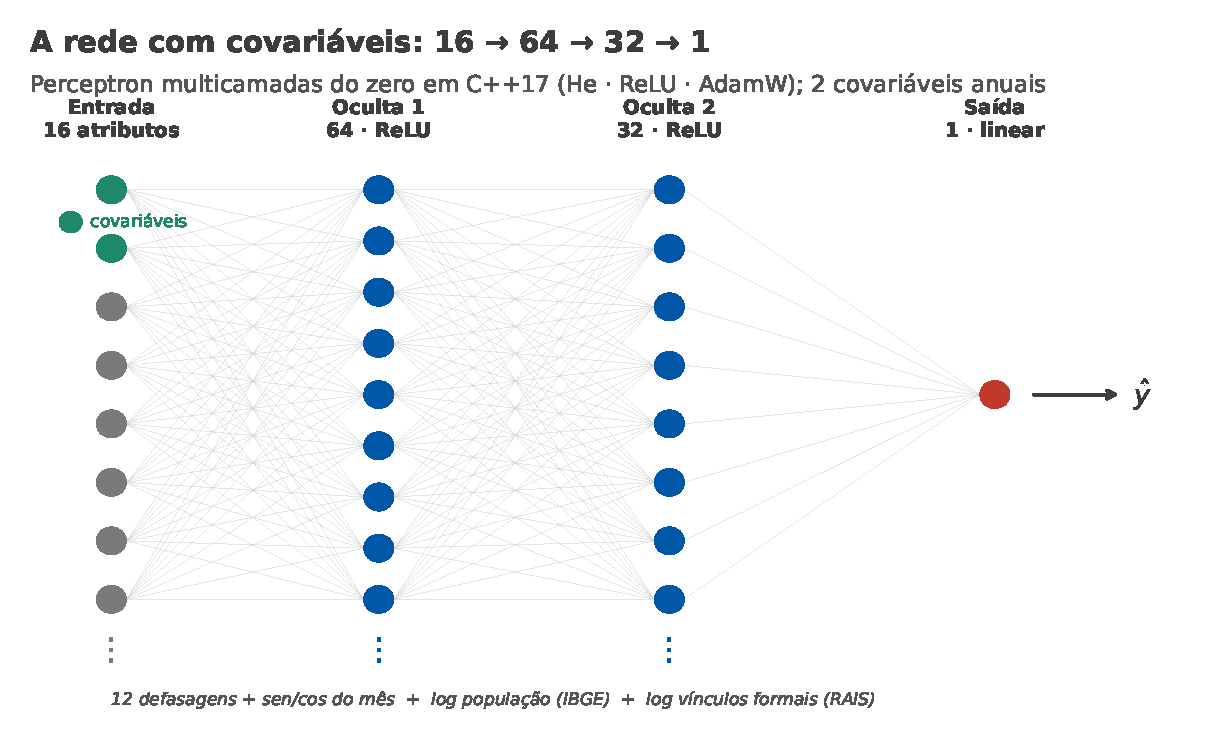
\includegraphics[width=0.95\textwidth]{fig10_arquitetura.pdf}
\caption{\textbf{Arquitetura da rede profunda com covariáveis
($16\to 64\to 32\to 1$).} Aos 14 atributos univariados juntam-se dois nós
de covariável (em verde): log da população (IBGE) e log dos vínculos
formais (RAIS). He, ReLU, AdamW; tudo do zero em C++17.}
\label{fig:arquitetura}
\end{figure}

\subsection{Inicialização sensível à variância}

Para redes ReLU, He \emph{et al.}~\C{ref:he} mostraram que preservar a
variância da ativação exige variância de peso $2/n_{\text{in}}$:
\begin{equation}
W^{(l)}_{ij}\sim\mathcal{N}\!\Bigl(0,\;\tfrac{2}{n_{l-1}}\Bigr),
\qquad b^{(l)}_i=0 ,
\label{eq:he}
\end{equation}
generalização, para ReLU, da inicialização de Glorot e
Bengio~\C{ref:glorot}.

\subsection{Perda e retropropagação}

A perda por exemplo é o erro quadrático sobre o alvo padronizado,
$\ell=(\widehat{y}-y)^2$, e $\mathcal{L}=\frac1N\sum_i(\widehat{y}_i-y_i)^2$.
O gradiente segue por retropropagação~\C{ref:rumelhart}. Com saída linear,
$\delta^{(L)}=2(\widehat{y}-y)$, e
\begin{equation}
\bm\delta^{(l)} = \Bigl(\bm W^{(l+1)\top}\bm\delta^{(l+1)}\Bigr)\odot\phi'\!\bigl(\bm z^{(l)}\bigr),
\qquad
\frac{\partial\ell}{\partial \bm W^{(l)}} = \bm\delta^{(l)}\bm a^{(l-1)\top},
\qquad
\frac{\partial\ell}{\partial \bm b^{(l)}} = \bm\delta^{(l)} ,
\label{eq:backprop}
\end{equation}
onde $\odot$ é o produto de Hadamard. A implementação acumula gradientes ao
longo de um minilote e dá um passo de otimização sobre o gradiente médio;
o fator $2$ é absorvido na taxa de aprendizado.

\subsection{Otimizador: AdamW}

Atualizamos com Adam~\C{ref:adam}, que adapta o passo por parâmetro a
partir de estimativas dos momentos do gradiente. Com $\bm g_t$ o gradiente
médio do minilote,
\begin{align}
\bm m_t &= \beta_1\bm m_{t-1} + (1-\beta_1)\,\bm g_t, &
\bm v_t &= \beta_2\bm v_{t-1} + (1-\beta_2)\,\bm g_t^{\odot 2},\\
\widehat{\bm m}_t &= \frac{\bm m_t}{1-\beta_1^{\,t}}, &
\widehat{\bm v}_t &= \frac{\bm v_t}{1-\beta_2^{\,t}},
\end{align}
e o passo, com decaimento de peso \emph{desacoplado} de Loshchilov e
Hutter~\C{ref:adamw},
\begin{equation}
\bm\theta_t = \bm\theta_{t-1} - \eta\,\frac{\widehat{\bm m}_t}{\sqrt{\widehat{\bm v}_t}+\varepsilon}
\;-\; \eta\,\lambda\,\bm\theta_{t-1}.
\label{eq:adamw}
\end{equation}
O último termo encolhe os pesos diretamente, recuperando a interpretação
de regularização $L_2$ sob Adam. Usamos $\beta_1=0{,}9$, $\beta_2=0{,}999$,
$\varepsilon=10^{-8}$, minilotes de 256. As autorregressões lineares usam
cronograma fixo ($\eta=10^{-2}$, sem decaimento, 25 épocas); os perceptrons
profundos, $\eta=10^{-3}$, $\lambda=10^{-4}$ e até 60 épocas com parada
antecipada.

\subsection{Parada antecipada}

Para conter o sobreajuste dos modelos profundos, retemos 15\% do treino
como validação e monitoramos o MAE de validação em famílias; com
\emph{paciência} de cinco épocas, interrompemos e restauramos os pesos da
melhor época (Figura~\ref{fig:curva})~\C{ref:goodfellow}. As autorregressões
lineares dispensam o mecanismo.

\begin{figure}[H]
\centering
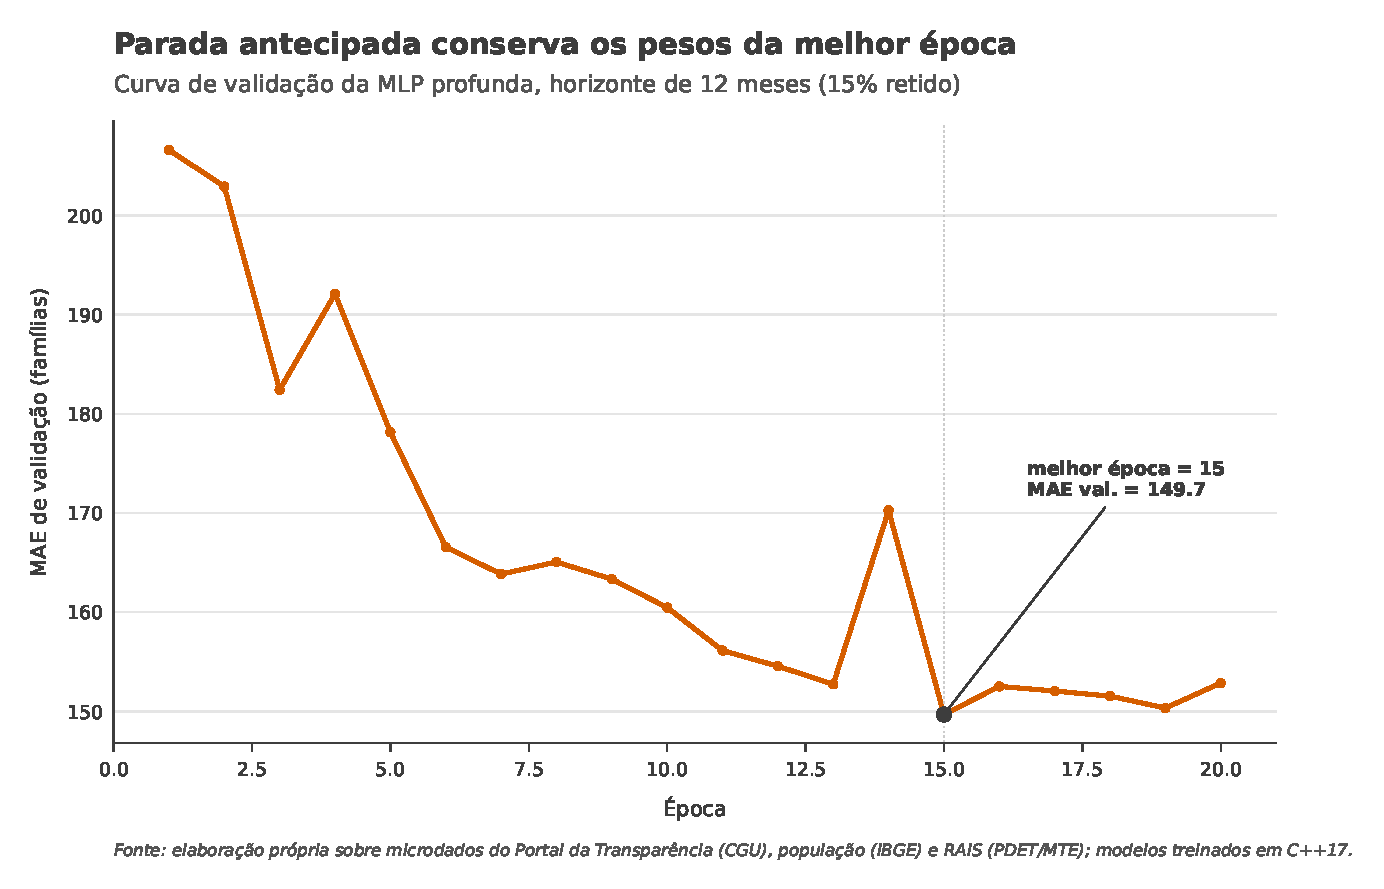
\includegraphics[width=0.91\textwidth]{fig06_curva_treino.pdf}
\caption{\textbf{Curva de validação do perceptron profundo ($H=12$).} O MAE
de validação cai, atinge um mínimo e oscila; a parada antecipada seleciona
e restaura os pesos da melhor época.}
\label{fig:curva}
\end{figure}

\subsection{Algoritmo de treino}

Reunindo as peças, o treino é o laço do Quadro~1: cada época
percorre o treino em minilotes de $B=256$; acumulam-se gradientes exemplo
a exemplo; ao fim do minilote, um passo de AdamW sobre o gradiente médio.

\begin{tcolorbox}[colback=black!2,colframe=black!35,boxrule=0.5pt,
  left=8pt,right=8pt,top=6pt,bottom=6pt,
  title=\textbf{Quadro 1 \textendash{} Treino com minilote AdamW e parada antecipada}]
\label{alg:treino}
\small\setstretch{1.12}
\begin{tabbing}
xx\=xx\=xx\=xxxxxxxxxxxxxxxxxxxxxxxxxxxxxxxxxx\kill
\textbf{entrada}: treino $\mathcal{D}$, validação $\mathcal{V}$ (15\%), épocas máx.\ $E$, paciência $p$\\
inicialize $\bm W,\bm b$ por He (eq.~\ref{eq:he}); $\bm m,\bm v\leftarrow 0$; $t\leftarrow 0$; $\bm\theta^\star\leftarrow\bm\theta$\\
\textbf{para} época $=1,\dots,E$ \textbf{faça}\\
\> embaralhe $\mathcal{D}$ e particione em minilotes de tamanho $B$\\
\> \textbf{para cada} minilote $\mathcal{B}$: avanço (eq.~\ref{eq:forward}); acumule grad.\ (eq.~\ref{eq:backprop});\\
\>\> $t\leftarrow t+1$; passo de AdamW (eq.~\ref{eq:adamw}); zere acumuladores\\
\> $\text{mae}_{\text{val}}\leftarrow$ MAE em $\mathcal{V}$, em famílias\\
\> \textbf{se} melhora \textbf{então} guarde $\bm\theta^\star\leftarrow\bm\theta$ \textbf{senão se} $p$ épocas sem melhora \textbf{então pare}\\
\textbf{retorne} $\bm\theta^\star$
\end{tabbing}
\end{tcolorbox}

\subsection{Um passo de treino, em números}

Para tornar concreto o maquinário das equações~\eqref{eq:forward}\textendash
\eqref{eq:adamw}, o Quadro~2 percorre um \emph{único}
exemplo da autorregressão linear: avanço, perda, gradiente e o primeiro
passo de AdamW de um peso. O exemplo ilustra por que a correção de viés do
Adam ($1-\beta_1^{\,t}$) importa nos primeiros passos e como o decaimento de
peso desacoplado encolhe o parâmetro independentemente do gradiente.

\begin{tcolorbox}[colback=black!2,colframe=black!35,boxrule=0.5pt,
  left=8pt,right=8pt,top=6pt,bottom=6pt,
  title=\textbf{Quadro 2 \textendash{} Um passo de AdamW para um peso (ilustrativo)}]
\small\setstretch{1.15}
Seja, no passo $t=1$, um peso $w=0{,}30$ cuja derivada da perda seja
$g=\partial\ell/\partial w=0{,}50$ (média do minilote), com
$\eta=10^{-2}$, $\beta_1=0{,}9$, $\beta_2=0{,}999$, $\varepsilon=10^{-8}$,
$\lambda=10^{-4}$.
\begin{align*}
m_1 &= 0{,}9\cdot 0 + 0{,}1\cdot 0{,}50 = 0{,}050, &
v_1 &= 0{,}999\cdot 0 + 0{,}001\cdot 0{,}50^2 = 2{,}5\times 10^{-4},\\
\widehat{m}_1 &= \tfrac{0{,}050}{1-0{,}9} = 0{,}50, &
\widehat{v}_1 &= \tfrac{2{,}5\times 10^{-4}}{1-0{,}999} = 0{,}25.
\end{align*}
\[
w \leftarrow w - \eta\,\frac{\widehat{m}_1}{\sqrt{\widehat{v}_1}+\varepsilon}
 - \eta\lambda w
 = 0{,}30 - 0{,}01\cdot\frac{0{,}50}{0{,}50} - 0{,}01\cdot 10^{-4}\cdot 0{,}30 \approx 0{,}290.
\]
A correção de viés transforma $m_1=0{,}05$ em $\widehat{m}_1=0{,}50$ (sem
ela, o primeiro passo seria dez vezes menor); o termo $-\eta\lambda w$
encolhe $w$ em $3\times 10^{-7}$, efeito minúsculo por passo mas cumulativo
ao longo das épocas.
\end{tcolorbox}

\subsection{Complexidade e número de parâmetros}

O custo de um avanço é dominado pelos produtos matriz-vetor:
$\mathrm{FLOPs}\approx 2\sum_l n_{l-1}n_l$. A Tabela~\ref{tab:modelos}
resume a anatomia dos cinco modelos. A contagem de parâmetros explicita o
argumento de viés-variância (Seção~\ref{sec:interpretacao}): as
autorregressões estimam 15\textendash 17 parâmetros; os perceptrons
profundos, mais de \num{3000}. As covariáveis acrescentam apenas dois
atributos \textemdash{} custo desprezível, sinal potencialmente grande.

\begin{table}[H]
\centering
\caption{Anatomia dos cinco modelos}
\label{tab:modelos}
\small
\begin{tabular}{@{}lrrl@{}}
\toprule
\textbf{Modelo} & \textbf{Parâmetros} & \textbf{FLOPs/avanço} & \textbf{Entrada / regularização} \\
\midrule
Persistência       & 0          & 0            & --- \\
AR linear          & 15         & 28           & 14 atrib.; fixo \\
MLP profunda       & \num{3073} & $\approx$\num{5888} & 14 atrib.; AdamW + parada antecip. \\
AR linear + cov.   & 17         & 32           & 16 atrib.; fixo \\
MLP profunda + cov.& \num{3201} & $\approx$\num{6144} & 16 atrib.; AdamW + parada antecip. \\
\bottomrule
\end{tabular}
\par\smallskip
{\footnotesize Parâmetros da MLP profunda: $14{\cdot}64{+}64+64{\cdot}32{+}32+32{\cdot}1{+}1=\num{3073}$;
com covariáveis, $16{\cdot}64{+}\cdots=\num{3201}$. Fonte: elaboração própria.}
\end{table}

\subsection{Implementação do zero em C++17}

Todo o motor \textemdash{} camadas densas, ReLU, retropropagação, AdamW
\textemdash{} é escrito à mão em C++17, usando apenas \texttt{<vector>},
\texttt{<cmath>}, \texttt{<map>} e \texttt{<random>}, sem LibTorch, BLAS ou
qualquer dependência de aprendizado profundo. Os pesos são armazenados em
ordem \emph{row-major} por camada; avanço e retropropagação operam um
exemplo por vez, acumulando o gradiente sobre o minilote antes de um passo
de Adam. Pedagogicamente alinhada a~\C{ref:chen-gupta}, a escolha torna
cada operação inspecionável e o experimento integralmente reproduzível, ao
custo de desempenho irrelevante nesta escala.

% =====================================================================
\section{Métricas e inferência}
\label{sec:metricas}
% =====================================================================

\subsection{Métricas de erro}

Todas as métricas são computadas \emph{em unidades de famílias}, após a
inversão da padronização, sobre as $\approx$\num{66504} previsões retidas de
cada horizonte. Para erros $e_i=\widehat{f}_i-f_i$,
\begin{align}
\mathrm{MAE}  &= \frac{1}{N}\sum_{i}\lvert e_i\rvert, &
\mathrm{MAPE} &= \frac{100}{N}\sum_{i}\frac{\lvert e_i\rvert}{f_i}, &
\mathrm{RMSE} &= \sqrt{\frac{1}{N}\sum_{i}e_i^2}, &
R^2 &= 1-\frac{\sum_i e_i^2}{\sum_i (f_i-\bar f)^2}.
\end{align}
O $R^2$ é dominado pela variância \emph{entre} municípios e, por isso,
pouco informativo aqui (fica acima de 0,98 para todos); a métrica que
separa os modelos é o MAPE, invariante de escala, complementada pelo MAE.

\subsection{Comparação pareada de modelos}

Com $n\approx\num{66504}$, qualquer diferença minúscula é
``estatisticamente significativa'' a um valor-$p$ desprezível; o
valor-$p$ isolado é desinformativo. Reportamos, por par de modelos,
pareados no mesmo conjunto: \emph{(i)} a diferença média de erro absoluto
$\Delta\mathrm{MAE}=\mathrm{MAE}_B-\mathrm{MAE}_A$ (positivo $\Rightarrow A$
vence), em famílias; \emph{(ii)} seu IC de 95\% por bootstrap pareado, com
\num{2000} reamostragens~\C{ref:efron}; \emph{(iii)} o valor-$p$ do teste
de Wilcoxon~\C{ref:wilcoxon}; e \emph{(iv)} a \emph{taxa de vitória}, a
fração de previsões em que $\lvert e_A\rvert\le\lvert e_B\rvert$. O
bootstrap mede a incerteza da \emph{magnitude}; Wilcoxon, a consistência do
\emph{sinal}; a taxa de vitória, sua \emph{disseminação}. A lógica de
comparar acurácia preditiva por pares remonta a Diebold e
Mariano~\C{ref:diebold}.

% =====================================================================
\section{Resultados: acurácia fora do tempo}
\label{sec:resultados}
% =====================================================================

A Tabela~\ref{tab:acuracia} reúne MAE e MAPE dos cinco modelos nos quatro
horizontes; a Figura~\ref{fig:mape} mostra o núcleo univariado e a
Figura~\ref{fig:ganho} traduz tudo em redução de MAE sobre a persistência.

\begin{table}[H]
\centering
\caption{Acurácia fora do tempo por horizonte ($\approx$\num{66504} previsões cada)}
\label{tab:acuracia}
\small
\begin{tabular}{@{}clrrr@{}}
\toprule
\textbf{Horizonte} & \textbf{Modelo} & \textbf{MAE (fam.)} & \textbf{MAPE (\%)} & \textbf{vs.\ persist.} \\
\midrule
\multirow{5}{*}{1 mês}
 & Persistência        & \textbf{54,6}  & 1,94 & --- \\
 & AR linear           & 57,5  & 1,98 & $-5\%$ \\
 & MLP profunda        & 54,9  & 2,04 & $-1\%$ \\
 & AR linear + cov.    & 60,3  & 1,98 & $-11\%$ \\
 & MLP profunda + cov. & 55,4  & \textbf{1,97} & $-2\%$ \\
\midrule
\multirow{5}{*}{3 meses}
 & Persistência        & 118,3 & 4,19 & --- \\
 & AR linear           & \textbf{98,1}  & 3,83 & $+17\%$ \\
 & MLP profunda        & 117,5 & 4,24 & $+1\%$ \\
 & AR linear + cov.    & 107,9 & \textbf{3,82} & $+9\%$ \\
 & MLP profunda + cov. & 125,2 & 4,22 & $-6\%$ \\
\midrule
\multirow{5}{*}{6 meses}
 & Persistência        & 206,1 & 7,26 & --- \\
 & AR linear           & 150,2 & 5,99 & $+27\%$ \\
 & MLP profunda        & 201,8 & 7,15 & $+2\%$ \\
 & AR linear + cov.    & \textbf{151,0} & \textbf{5,95} & $+27\%$ \\
 & MLP profunda + cov. & 189,1 & 6,62 & $+8\%$ \\
\midrule
\multirow{5}{*}{12 meses}
 & Persistência        & 268,8 & 9,92 & --- \\
 & AR linear           & 243,1 & 8,80 & $+10\%$ \\
 & MLP profunda        & 297,1 & 9,89 & $-11\%$ \\
 & \textbf{AR linear + cov.} & \textbf{223,3} & \textbf{8,62} & \textbf{$+17\%$} \\
 & MLP profunda + cov. & 298,7 & 9,55 & $-11\%$ \\
\bottomrule
\end{tabular}
\par\smallskip
{\footnotesize Em negrito, o melhor de cada bloco. A coluna ``vs.\
persist.'' é a redução de MAE sobre a ingênua. Fonte: elaboração própria.}
\end{table}

\begin{figure}[H]
\centering
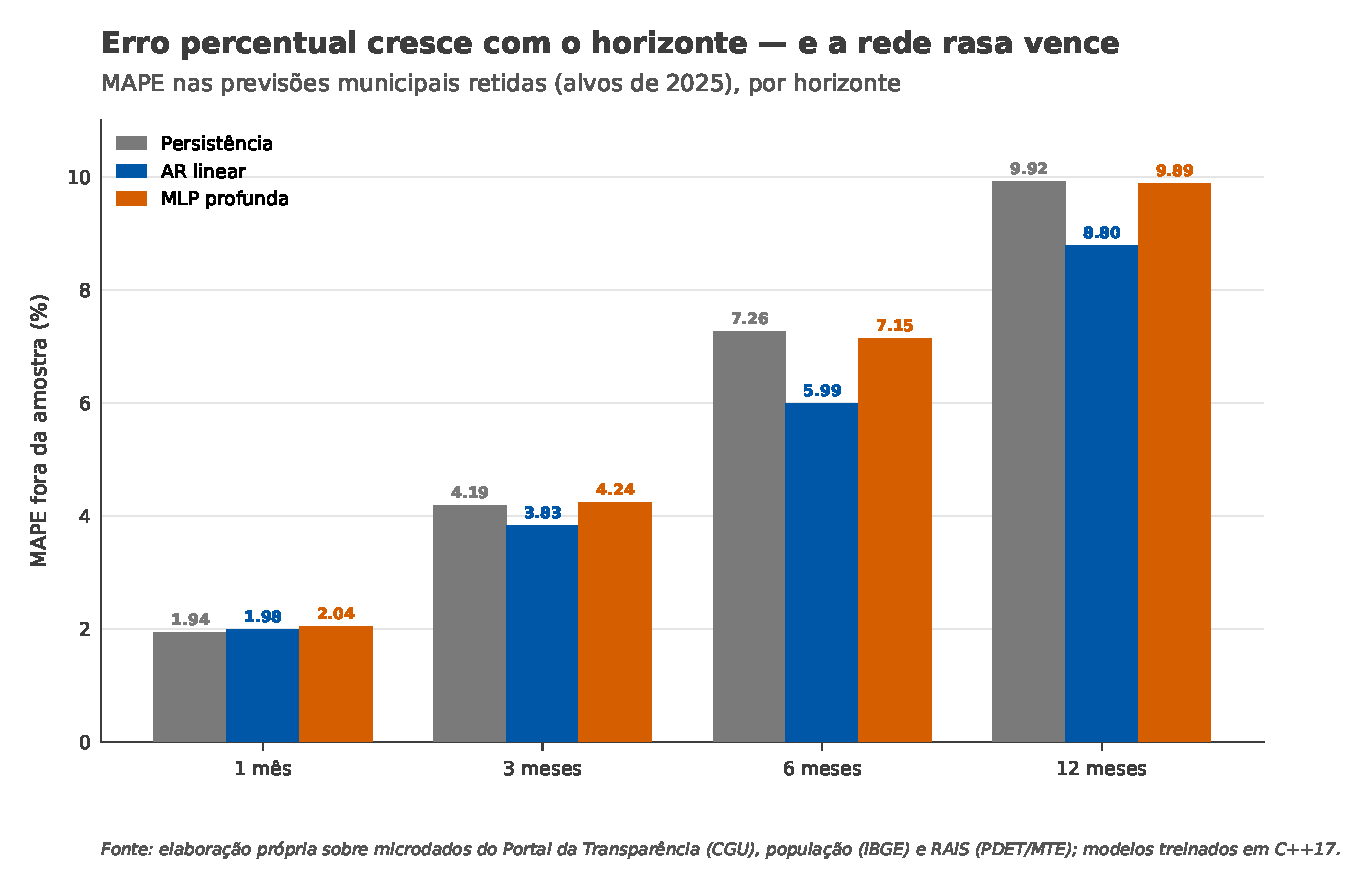
\includegraphics[width=0.95\textwidth]{fig02_mape_horizonte.pdf}
\caption{\textbf{MAPE fora da amostra (núcleo univariado).} A um mês a
persistência é imbatível; de três meses em diante a autorregressão linear
tem o menor erro percentual, e a vantagem cresce com o horizonte.}
\label{fig:mape}
\end{figure}

\begin{figure}[H]
\centering
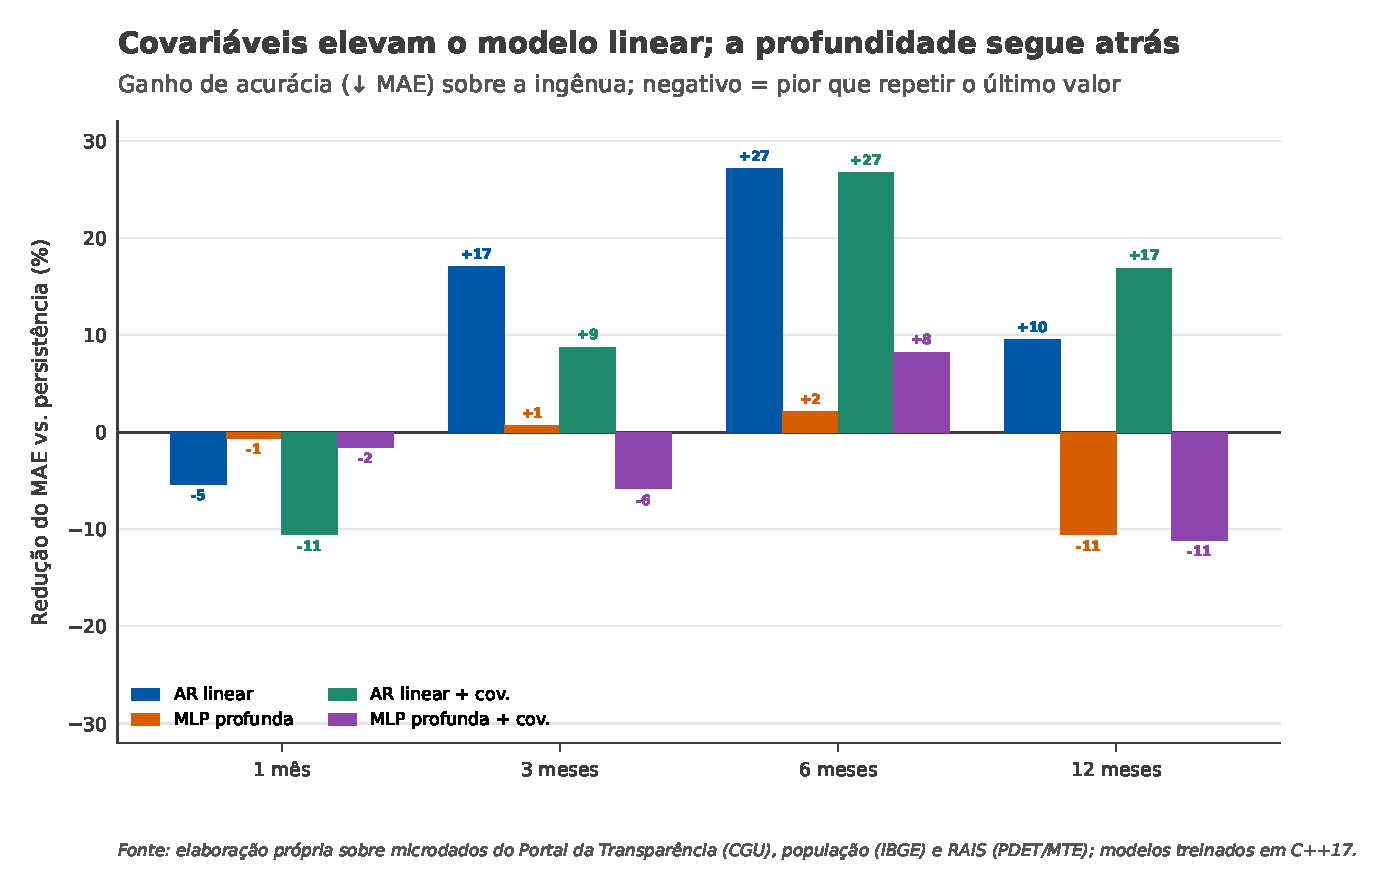
\includegraphics[width=0.95\textwidth]{fig03_ganho_mae.pdf}
\caption{\textbf{Redução de MAE sobre a persistência, quatro modelos
aprendidos.} A autorregressão linear (com e sem covariáveis) lidera; a
profundidade fica sistematicamente atrás. Em 12 meses, é o modelo
\emph{linear com covariáveis} que mais reduz o erro ($+17\%$).}
\label{fig:ganho}
\end{figure}

A leitura é direta. A \textbf{um mês}, a persistência tem o menor MAE
(54,6); nenhum modelo aprendido a supera \textemdash{} assinatura empírica
de um passeio aleatório. De \textbf{três meses} em diante, a autorregressão
linear assume a liderança: reduz o MAE em 17\%, 27\% e 10\% (3, 6 e 12
meses) sobre a ingênua. O perceptron profundo melhora pouco e é
\emph{dominado} pelo linear em todo horizonte; com ou sem covariáveis, a
profundidade não paga. O ponto novo, e o mais relevante, aparece no
horizonte de \textbf{doze meses}: ali o modelo \emph{linear com
covariáveis} é o melhor de todos ($+17\%$ vs.\ $+10\%$ do linear
univariado), sinal de que demografia e emprego carregam informação
estrutural que o histórico recente não contém. A próxima seção isola esse
efeito.

% =====================================================================
\section{O efeito das covariáveis}
\label{sec:efeito}
% =====================================================================

A pergunta-chave do estudo multivariado é direta: \emph{adicionar
população e emprego formal melhora a previsão?} A
Figura~\ref{fig:efeito} responde, mostrando o $\Delta$MAE de cada modelo
\emph{com} covariáveis contra sua versão univariada, com IC de 95\%; a
Tabela~\ref{tab:efeito} traz os números.

\begin{table}[H]
\centering
\caption{Efeito das covariáveis: $\Delta$MAE (com cov.\ $-$ univariado), pareado}
\label{tab:efeito}
\small
\begin{tabular}{@{}clrc@{}}
\toprule
\textbf{$H$} & \textbf{Comparação} & \textbf{$\Delta$MAE (fam.)} & \textbf{IC 95\%} \\
\midrule
\multirow{2}{*}{1}  & linear+cov vs.\ linear & $-2{,}85$ & $[-5{,}4;\,-0{,}3]$ \\
                    & deep+cov vs.\ deep     & $-0{,}50$ & $[-1{,}6;\,+0{,}5]$ \\
\midrule
\multirow{2}{*}{3}  & linear+cov vs.\ linear & $-9{,}81$ & $[-12{,}4;\,-7{,}2]$ \\
                    & deep+cov vs.\ deep     & $-7{,}70$ & $[-10{,}4;\,-5{,}2]$ \\
\midrule
\multirow{2}{*}{6}  & linear+cov vs.\ linear & $-0{,}82$ & $[-2{,}1;\,+0{,}5]$ \\
                    & \textbf{deep+cov vs.\ deep} & \boldmath$+12{,}71$ & $[+8{,}4;\,+16{,}7]$ \\
\midrule
\multirow{2}{*}{12} & \textbf{linear+cov vs.\ linear} & \boldmath$+19{,}76$ & $[+12{,}1;\,+27{,}5]$ \\
                    & deep+cov vs.\ deep     & $-1{,}55$ & $[-5{,}9;\,+3{,}1]$ \\
\bottomrule
\end{tabular}
\par\smallskip
{\footnotesize $\Delta$MAE${}>0$ indica que as covariáveis \emph{ajudam}.
IC por bootstrap pareado (\num{2000} reamostragens). Fonte: elaboração própria.}
\end{table}

\begin{figure}[H]
\centering
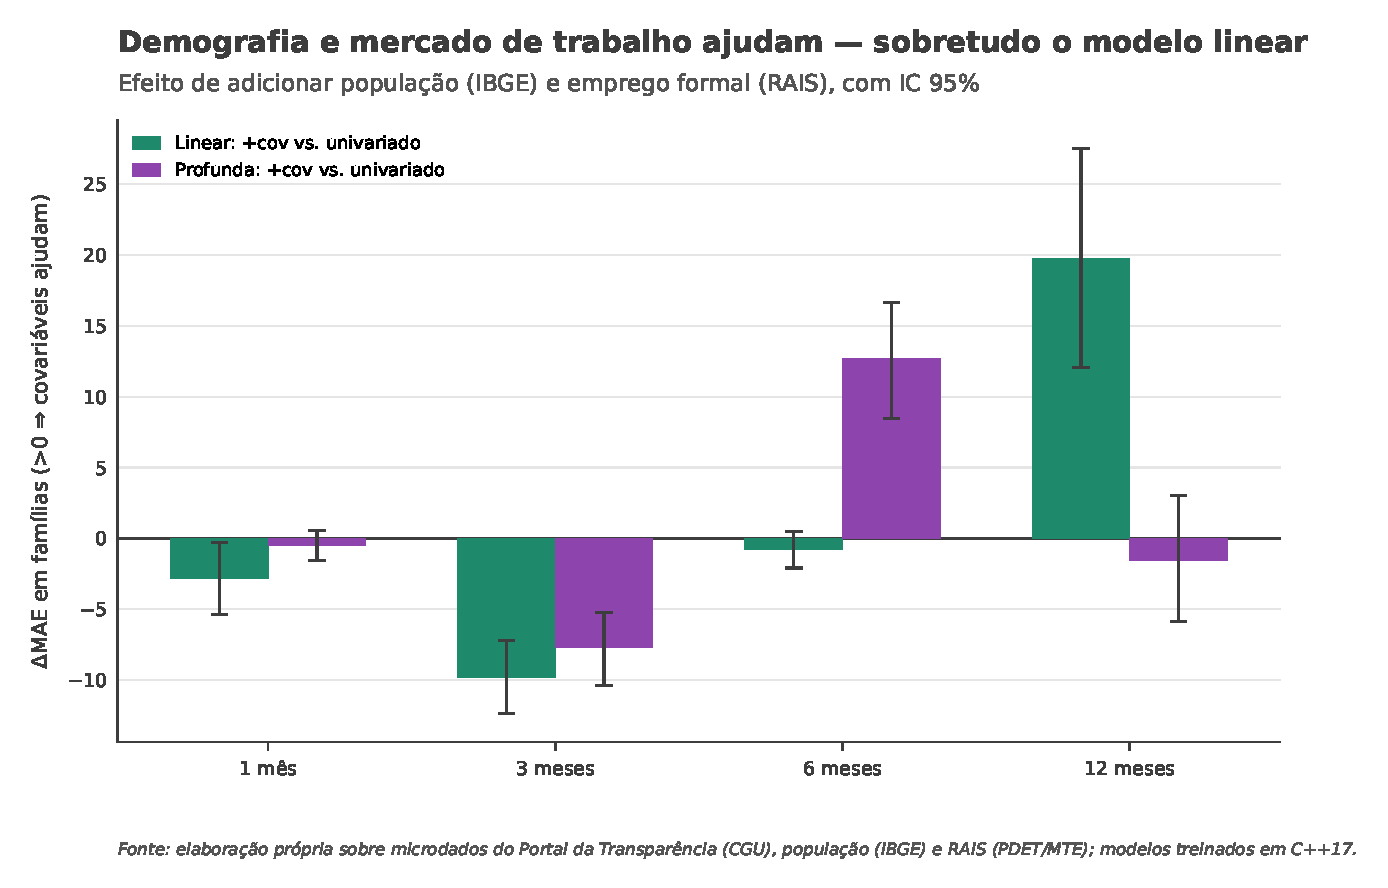
\includegraphics[width=0.95\textwidth]{fig05_efeito_covariaveis.pdf}
\caption{\textbf{O valor das covariáveis cresce com o horizonte.}
$\Delta$MAE de adicionar população e emprego formal, com IC 95\%: negativo
ou nulo a 1\textendash 3 meses, fortemente positivo para o modelo linear
em 12 meses ($+19{,}8$, IC $[+12{,}1;+27{,}5]$) e para o profundo em 6
meses ($+12{,}7$).}
\label{fig:efeito}
\end{figure}

O padrão é claro e econômico. A \textbf{curto prazo (1\textendash 3
meses)}, as covariáveis \emph{não ajudam} e chegam a prejudicar
\textemdash{} a dinâmica é dominada pela autocorrelação mensal, e
variáveis anuais defasadas apenas adicionam ruído e uma incompatibilidade
de frequência. A \textbf{seis meses}, ajudam o modelo profundo de forma
robusta ($+12{,}7$). A \textbf{doze meses}, elevam o modelo linear de forma
grande e robusta ($+19{,}8$, IC estritamente positivo): é justamente onde a
autorregressão pura enfraquece e os motores estruturais \textemdash{}
quantos habitantes, quantos empregos formais \textemdash{} passam a
governar a demanda. O valor de uma covariável de baixa frequência é,
portanto, \emph{função do horizonte}: invisível no curto prazo, decisivo no
longo. Notavelmente, mesmo alimentada com covariáveis, a rede profunda
permanece atrás do modelo linear (Tabela~\ref{tab:acuracia}): a informação
ajuda, mas a forma certa de usá-la continua sendo o modelo parcimonioso.

% =====================================================================
\section{Significância estatística}
\label{sec:significancia}
% =====================================================================

A Tabela~\ref{tab:sig} compara os modelos aprendidos contra a persistência
e entre si; a Figura~\ref{fig:ci} visualiza a vantagem da autorregressão
linear com IC; a Figura~\ref{fig:winrate}, a taxa de vitória; e a
Figura~\ref{fig:ecdf}, a distribuição completa do erro em seis meses.

\begin{table}[H]
\centering
\caption{Comparações pareadas selecionadas ($n\approx\num{66504}$)}
\label{tab:sig}
\small
\begin{tabular}{@{}clrc@{}}
\toprule
\textbf{$H$} & \textbf{Comparação} & \textbf{$\Delta$MAE (fam.)} & \textbf{IC 95\%} \\
\midrule
\multirow{2}{*}{3}
 & AR linear vs.\ persist. & $+20{,}18$ & $[+17{,}6;\,+22{,}7]$ \\
 & AR linear vs.\ deep     & $+19{,}39$ & $[+16{,}8;\,+22{,}0]$ \\
\midrule
\multirow{2}{*}{6}
 & \textbf{AR linear vs.\ persist.} & \boldmath$+56{,}00$ & $[+49{,}7;\,+62{,}4]$ \\
 & deep+cov vs.\ AR linear & $-38{,}95$ & $[-44{,}7;\,-33{,}6]$ \\
\midrule
\multirow{2}{*}{12}
 & AR linear vs.\ persist. & $+25{,}71$ & $[+14{,}2;\,+37{,}9]$ \\
 & AR linear + cov.\ vs.\ persist. & $+45{,}5$ & $[+33;\,+58]$ \\
\bottomrule
\end{tabular}
\par\smallskip
{\footnotesize $\Delta$MAE${}>0$ favorece o primeiro modelo. Todos os
testes de Wilcoxon têm $p<10^{-30}$; a leitura está no IC. A última linha é
a soma das vantagens linear vs.\ persist.\ ($+25{,}71$) e linear+cov vs.\
linear ($+19{,}76$). Fonte: elaboração própria.}
\end{table}

\begin{figure}[H]
\centering
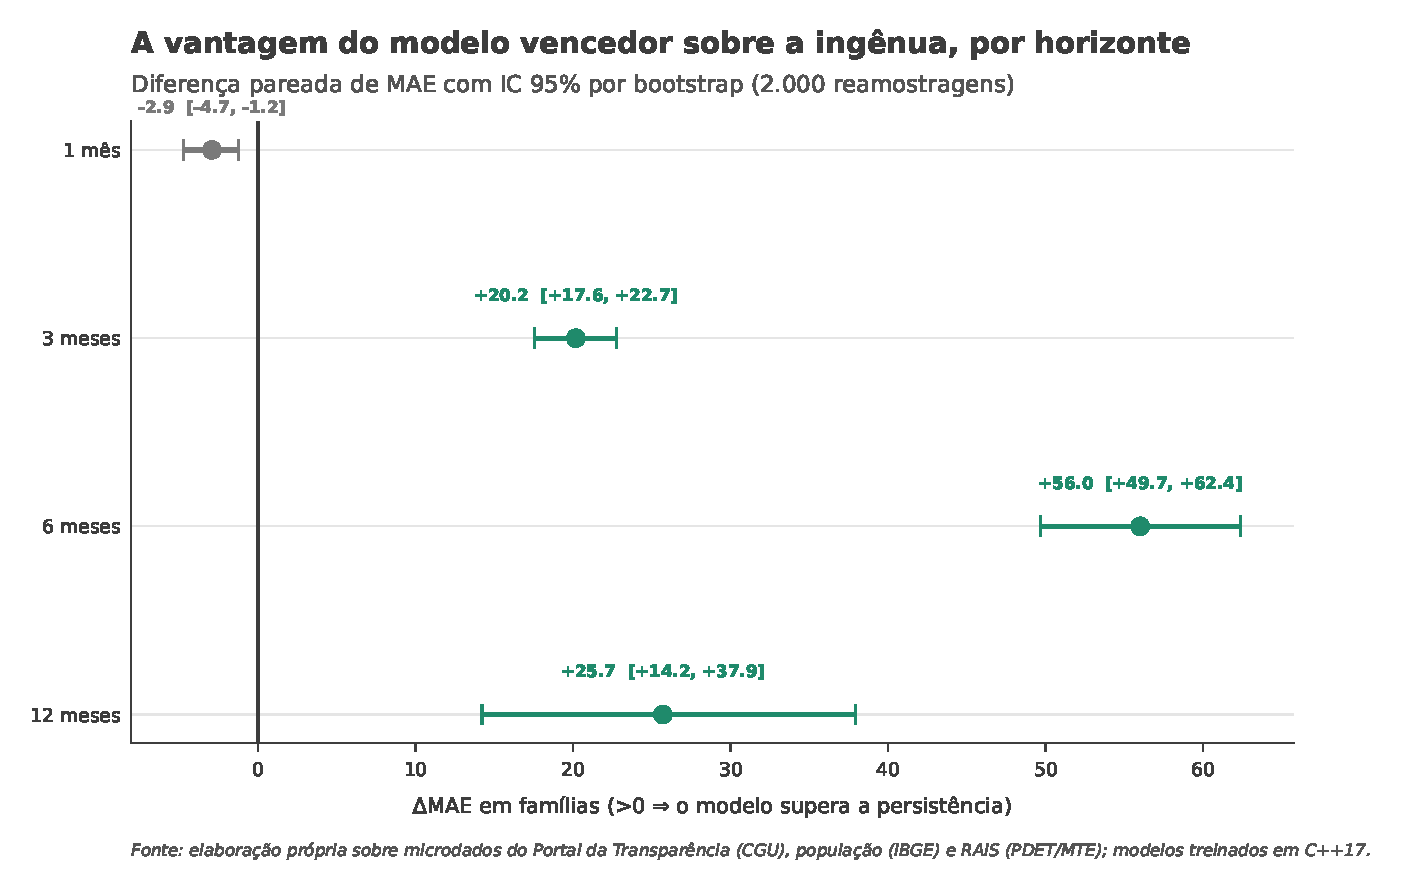
\includegraphics[width=0.95\textwidth]{fig04_delta_ci.pdf}
\caption{\textbf{Vantagem da autorregressão linear sobre a persistência,
com IC 95\%.} A seis meses o intervalo é estritamente positivo e largo
($+56$ famílias): vantagem grande e robusta. A doze meses permanece
positivo, e as covariáveis o ampliam ainda mais (Seção~\ref{sec:efeito}).}
\label{fig:ci}
\end{figure}

\begin{figure}[H]
\centering
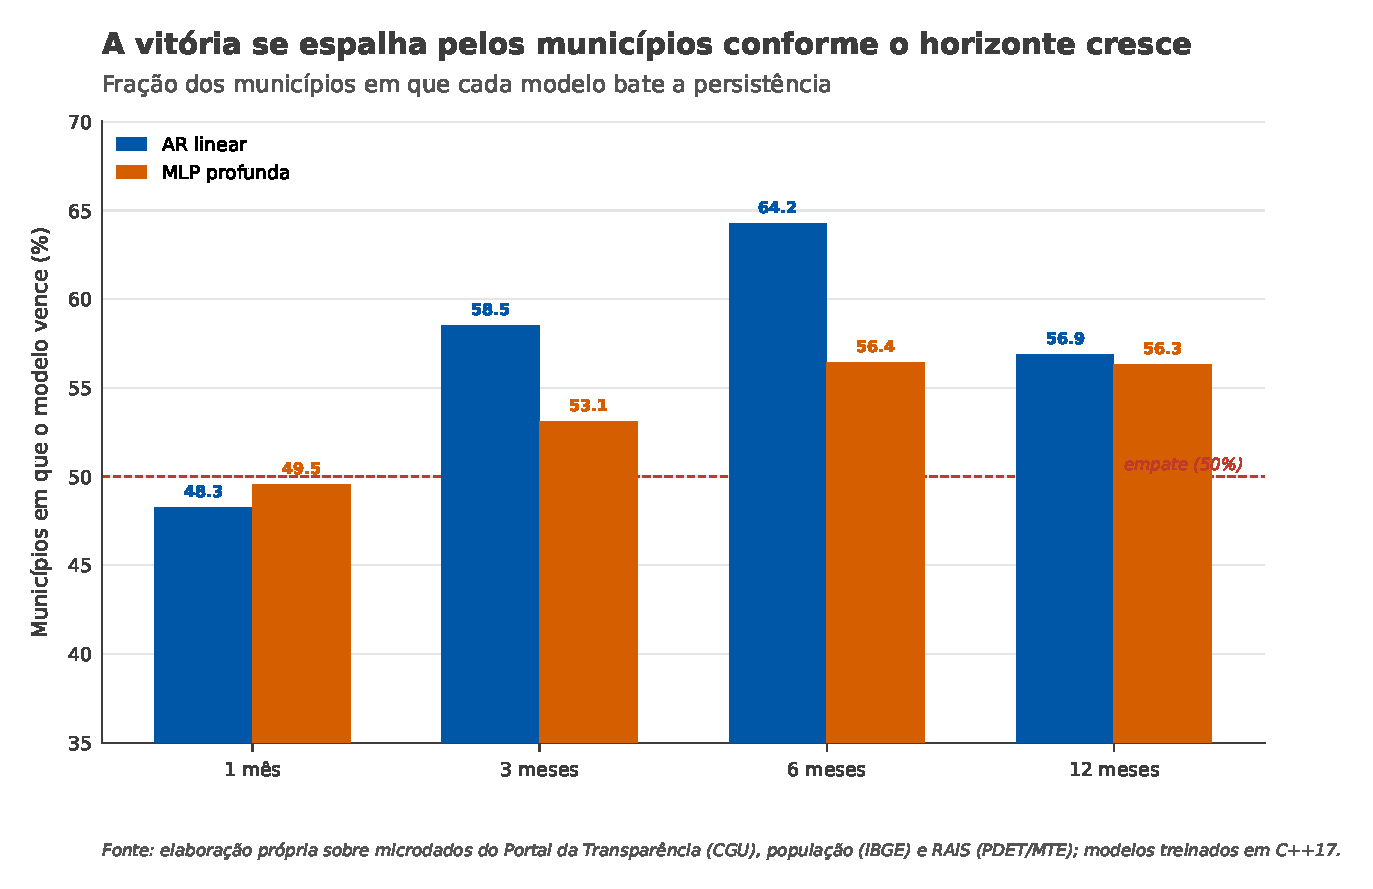
\includegraphics[width=0.95\textwidth]{fig07_winrate.pdf}
\caption{\textbf{Taxa de vitória sobre a persistência.} A fração de
municípios em que cada modelo vence cresce com o horizonte, atingindo
64\% para a autorregressão linear em seis meses: a vantagem se dissemina
pela maioria, não vem de poucos atípicos.}
\label{fig:winrate}
\end{figure}

\begin{figure}[H]
\centering
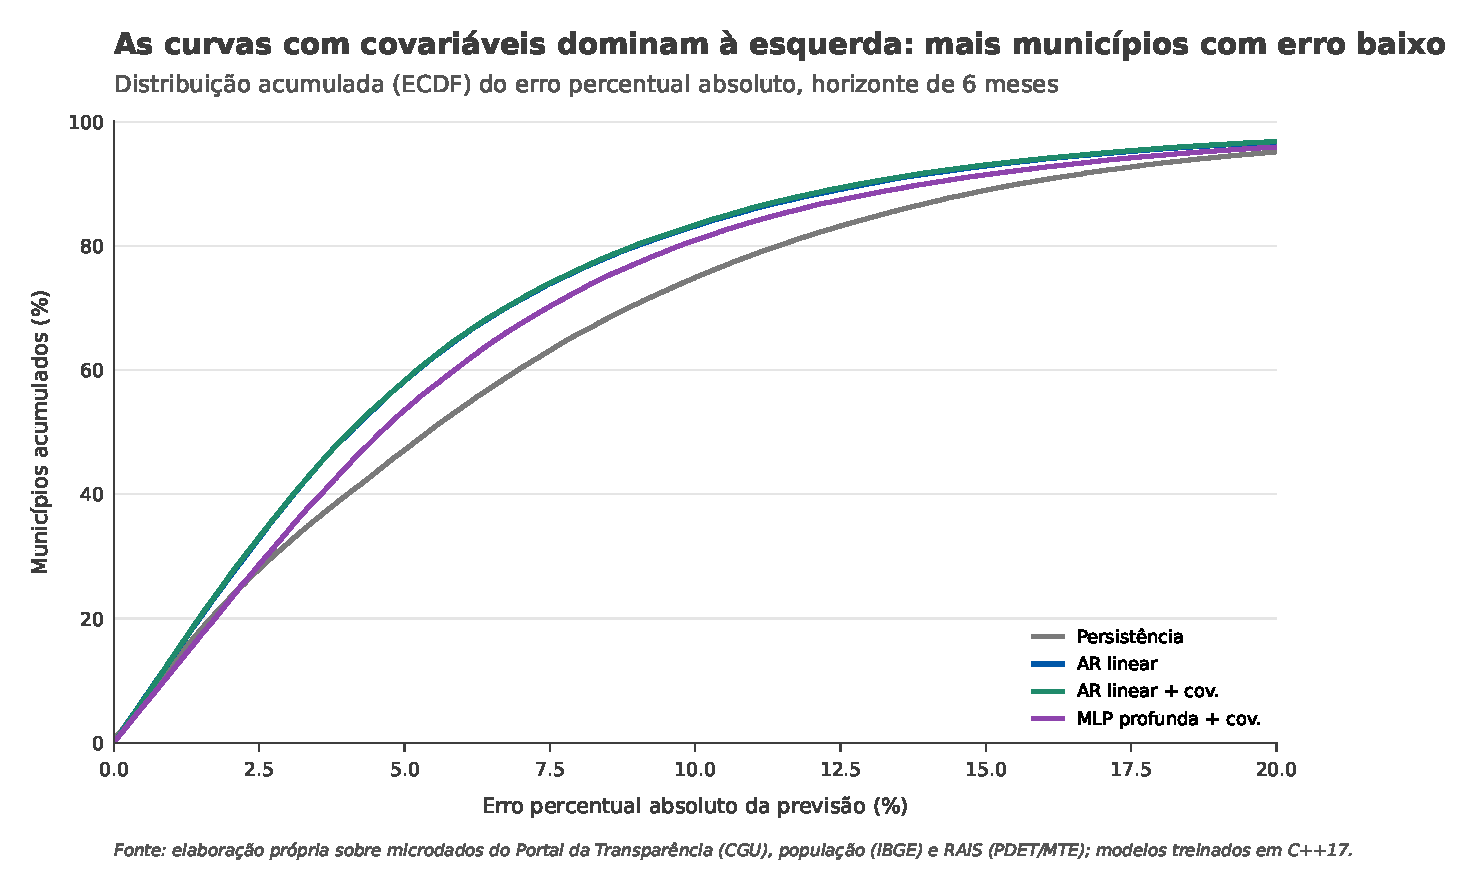
\includegraphics[width=0.95\textwidth]{fig08_ecdf_erro.pdf}
\caption{\textbf{Distribuição acumulada do erro percentual absoluto
($H=6$).} As curvas com covariáveis e a do modelo linear ficam à esquerda
da persistência em quase toda a faixa: para qualquer limiar de erro, mais
municípios o cumprem. Domínio estocástico de primeira ordem aproximado.}
\label{fig:ecdf}
\end{figure}

\subsection{Síntese e robustez}

A Tabela~\ref{tab:sintese} resume o melhor modelo em cada horizonte e o
ganho correspondente. A conclusão é \emph{robusta} a múltiplos critérios:
as quatro lentes \textemdash{} MAE, MAPE (Tabela~\ref{tab:acuracia}), RMSE
($R^2$, Apêndice~A) e taxa de vitória (Apêndice~B) \textemdash{} concordam
na ordenação dos modelos em 3, 6 e 12 meses, e os intervalos de confiança
das vantagens decisivas são estritamente positivos. Nenhuma das conclusões
depende de uma única métrica ou de um único horizonte.

\begin{table}[H]
\centering
\caption{Síntese: melhor modelo por horizonte}
\label{tab:sintese}
\small
\begin{tabular}{@{}clrl@{}}
\toprule
\textbf{Horizonte} & \textbf{Melhor modelo} & \textbf{Redução de MAE} & \textbf{Regime} \\
\midrule
1 mês   & Persistência       & ---     & passeio aleatório \\
3 meses & AR linear          & $+17\%$ & autocorrelação domina \\
6 meses & AR linear (+ cov.) & $+27\%$ & ganho máximo da AR \\
12 meses& AR linear + cov.   & $+17\%$ & covariáveis decisivas \\
\bottomrule
\end{tabular}
\par\smallskip
{\footnotesize Redução de MAE sobre a persistência. Em 6 meses, AR linear e
AR linear + cov.\ empatam ($+27\%$). Fonte: elaboração própria.}
\end{table}

Conclusões inferenciais. \emph{(i)} A vantagem da autorregressão linear em
seis meses é grande, robusta e disseminada (vence 64\% dos municípios).
\emph{(ii)} A doze meses a vantagem persiste e é \emph{ampliada pelas
covariáveis}: linear+cov supera a persistência por $\approx{+}45$ famílias,
contra $+26$ do linear puro. \emph{(iii)} A profundidade, mesmo com
covariáveis, é dominada pela autorregressão linear em 3, 6 e 12 meses
(deep+cov vs.\ linear: $-27$, $-39$, $-56$ famílias) \textemdash{} a
informação ajuda, a capacidade extra não.

% =====================================================================
\section{Interpretação: quando ajudam a profundidade e as covariáveis?}
\label{sec:interpretacao}
% =====================================================================

Dois fenômenos pedem explicação: por que a rede mais simples vence a mais
profunda, e por que o valor das covariáveis cresce com o horizonte. Ambos
seguem da estrutura do sinal e do compromisso entre viés e
variância~\C{ref:goodfellow}, \C{ref:hyndman}.

\subsection{Por que a profundidade não paga}

\textbf{A um mês, a série é quase um passeio aleatório.} A melhor previsão
de $f_{c,t}$ a partir de $f_{c,t-1}$ é aproximadamente o próprio
$f_{c,t-1}$; o incremento é dominado por ruído. A persistência é quase
ótima, e qualquer parâmetro estimado só adiciona variância.
\textbf{Num sinal quase log-linear, a autorregressão é o modelo do
tamanho certo.} Uma combinação linear de doze defasagens captura quase
toda a estrutura previsível \textemdash{} tendência e persistência
\textemdash{} com pouquíssimos parâmetros, e generaliza melhor fora do
tempo. \textbf{O perceptron profundo gasta capacidade que o sinal não
recompensa:} suas camadas ocultas modelam interações não-lineares; quando
a estrutura é quase linear, a capacidade extra vira variância
(sobreajuste), não redução de viés. A regularização o resgata, mas não o
suficiente para alcançar o linear.

\subsection{Uma leitura formal: viés, variância e horizonte}

Para um estimador $\widehat{f}$ de $f=g(\bm x)+\epsilon$ com ruído de média
zero e variância $\sigma^2$, o erro quadrático esperado se decompõe como
\begin{equation}
\mathbb{E}\bigl[(f-\widehat{f})^2\bigr]
= \underbrace{\bigl(g-\mathbb{E}[\widehat{f}]\bigr)^2}_{\text{viés}^2}
+ \underbrace{\mathbb{E}\bigl[(\widehat{f}-\mathbb{E}[\widehat{f}])^2\bigr]}_{\text{variância}}
+ \underbrace{\sigma^2}_{\text{irredutível}} .
\label{eq:bv}
\end{equation}
A persistência tem viés alto e variância nula; a autorregressão linear
corta o viés com variância pequena; o perceptron profundo reduz mais o
viés \emph{em princípio}, mas adiciona variância substancial. O ponto que
minimiza~\eqref{eq:bv} \emph{depende do horizonte}: em $H=1$, o termo
$\sigma^2$ domina e vence quem nada estima (persistência); em $H=6$, o viés
da persistência explode e a autorregressão acerta o equilíbrio.

\subsection{Por que o valor das covariáveis cresce com o horizonte}

A mesma equação~\eqref{eq:bv} explica o efeito das covariáveis. A
informação que uma covariável adiciona reduz o viés \emph{na medida em que
ela prediz a parte do alvo que as defasagens não predizem}. A curto prazo,
as defasagens já contêm quase tudo: a população de um município há um ano
nada acrescenta sobre o próximo mês, e a covariável anual, defasada, apenas
injeta variância \textemdash{} daí o $\Delta$MAE negativo em
1\textendash 3 meses (Tabela~\ref{tab:efeito}). A longo prazo, porém, a
autocorrelação se esgota e a previsão precisa de \emph{âncoras
estruturais}: quantos habitantes, quanto emprego formal. É aí que a
covariável corta viés genuíno, e o $\Delta$MAE se torna grande e positivo
em 12 meses. Em suma: o valor de uma covariável de baixa frequência é
crescente no horizonte porque é exatamente no longo prazo que o sinal
autorregressivo se torna insuficiente.

A lição metodológica \textemdash{} \emph{case a capacidade do modelo e a
frequência da informação à estrutura e ao horizonte do problema}
\textemdash{} ecoa, em dados públicos brasileiros, o achado das competições
de previsão em larga escala~\C{ref:m4}: sofisticação não é, por si,
acurácia.

% =====================================================================
\section{Projeção 2026\textendash 2028}
\label{sec:projecao}
% =====================================================================

\subsection{Procedimento e o porquê de o agregado ser mais fácil}

Para projetar, reajustamos os modelos sobre \emph{todas} as janelas
observadas e rolamos cada município adiante de forma \emph{recursiva}: cada
previsão vira a entrada mais recente da janela seguinte; as covariáveis são
mantidas no último ano conhecido (2024), por ainda não observadas no
futuro. Somamos as previsões municipais à trajetória nacional
$\widehat{N}_t=\sum_c\widehat{f}_{c,t}$. A incerteza nacional é o MAPE
\emph{agregado} de backtest, não a soma dos erros municipais, porque na
agregação os erros idiossincráticos largamente se cancelam. Formalmente,
para erros $e_c$ com variância $\varsigma_c^2$ e correlação $\rho_{cc'}$,
\begin{equation}
\mathrm{Var}\Bigl(\textstyle\sum_c e_c\Bigr)
= \sum_c \varsigma_c^2 + \sum_{c\neq c'}\rho_{cc'}\,\varsigma_c\,\varsigma_{c'} ;
\label{eq:varsoma}
\end{equation}
como $\rho_{cc'}$ é, em média, pequeno, o desvio do agregado cresce como
$\sqrt{m}$ enquanto o agregado cresce como $m$, e o erro relativo encolhe
$\sim 1/\sqrt{m_{\text{ef}}}$. É por isso que o MAPE nacional cai para
1,29\% / 2,17\% / 3,52\% / 4,68\% (modelo linear) em 1 / 3 / 6 / 12 meses
\textemdash{} muito abaixo dos MAPEs municipais
(Tabela~\ref{tab:acuracia}). A Figura~\ref{fig:ajuste} mostra o ajuste
nacional sobre 2025, com as covariáveis reduzindo ainda mais o erro
agregado de longo prazo (MAPE nacional de 4,49\% em 12 meses para o modelo
linear com covariáveis).

\begin{figure}[H]
\centering
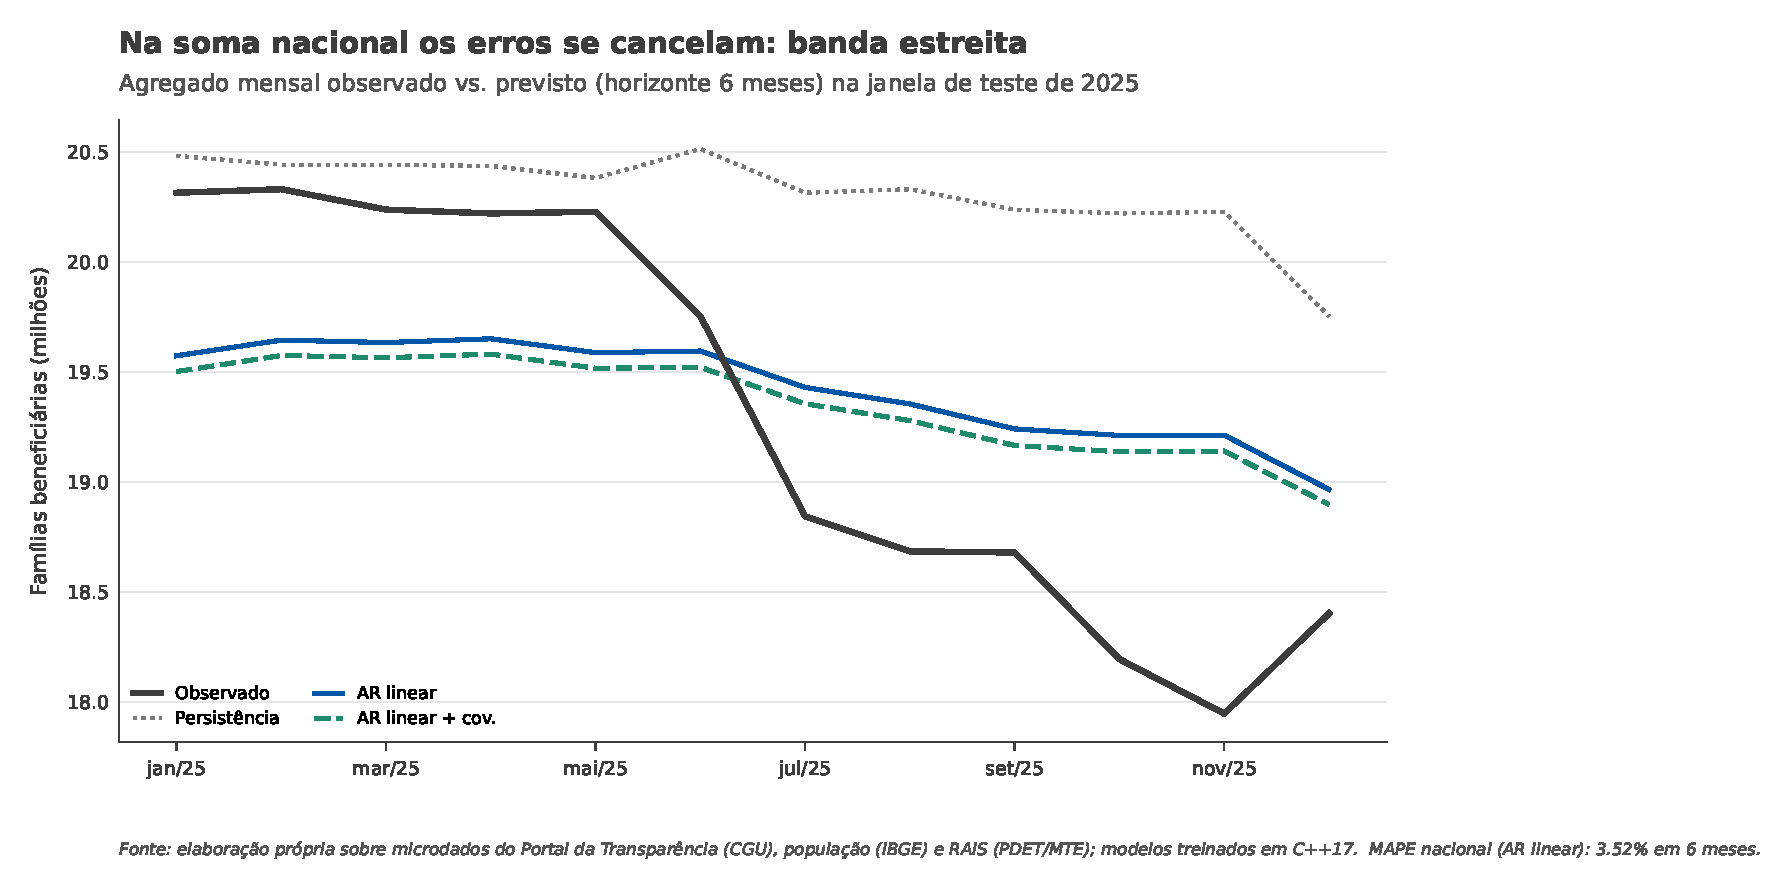
\includegraphics[width=0.95\textwidth]{fig09_ajuste_nacional_h6.pdf}
\caption{\textbf{Ajuste nacional na janela de teste ($H=6$).} A soma das
previsões municipais reproduz o agregado observado de 2025 com erro
pequeno; os erros municipais cancelam-se na agregação, o que justifica
usar o MAPE nacional como banda da projeção.}
\label{fig:ajuste}
\end{figure}

\subsection{Propagação de erro na recursão}

A projeção a $k$ meses encadeia $k$ previsões de um passo, cada uma
alimentada pela anterior. Se cada passo introduz um erro
$\eta_t$ aproximadamente de média zero e variância $\sigma_\eta^2$, e o
operador de um passo tem ganho local $|a|<1$ (a série é estacionária em
torno de sua tendência na escala padronizada), o erro acumulado após $k$
passos satisfaz, em primeira ordem,
\begin{equation}
\varepsilon_k \approx \sum_{j=0}^{k-1} a^{\,j}\,\eta_{k-j},
\qquad
\mathrm{Var}(\varepsilon_k) \approx \sigma_\eta^2\,\frac{1-a^{2k}}{1-a^2}
\xrightarrow[k\to\infty]{} \frac{\sigma_\eta^2}{1-a^2}.
\label{eq:recursao}
\end{equation}
Dois efeitos competem. De um lado, a variância do erro \emph{cresce} com o
horizonte, mas \emph{satura} (não explode), porque $|a|<1$ amortece
contribuições antigas. De outro, esse mesmo amortecimento implica
\emph{reversão à média}: previsões de longo prazo são puxadas para a média
histórica de cada município, o que tende a suavizar trajetórias e pode
subestimar movimentos persistentes \textemdash{} é a origem da limitação
discutida na Seção~\ref{sec:limitacoes}. A equação~\eqref{eq:recursao}
explica por que a banda nacional da Figura~\ref{fig:serie} se alarga de
forma decrescente, e não linear, com o horizonte.

\subsection{Resultados da projeção}

A Figura~\ref{fig:serie} apresenta a série histórica e a projeção até
dezembro de 2028; a Tabela~\ref{tab:projecao} resume os marcos. A carga de
casos nacional atingiu o \textbf{pico em janeiro de 2023}
(\num{21243010} famílias) e \textbf{recua desde então}, em
\num{18401764} famílias em dezembro de 2025. Ambos os modelos projetam
\emph{consolidação, não crescimento}. A trajetória central
(autorregressão linear) leva a $\approx\num{15442971}$ famílias em
dezembro de 2028 ($-16\%$ ante dezembro de 2025); o modelo linear com
covariáveis projeta praticamente o mesmo ($\approx\num{15456747}$), e o
perceptron profundo com covariáveis, um recuo mais brando
($\approx\num{15902025}$). A convergência das projeções para a faixa de
15,4\textendash 15,9 milhões reforça a robustez da conclusão.

\begin{figure}[H]
\centering
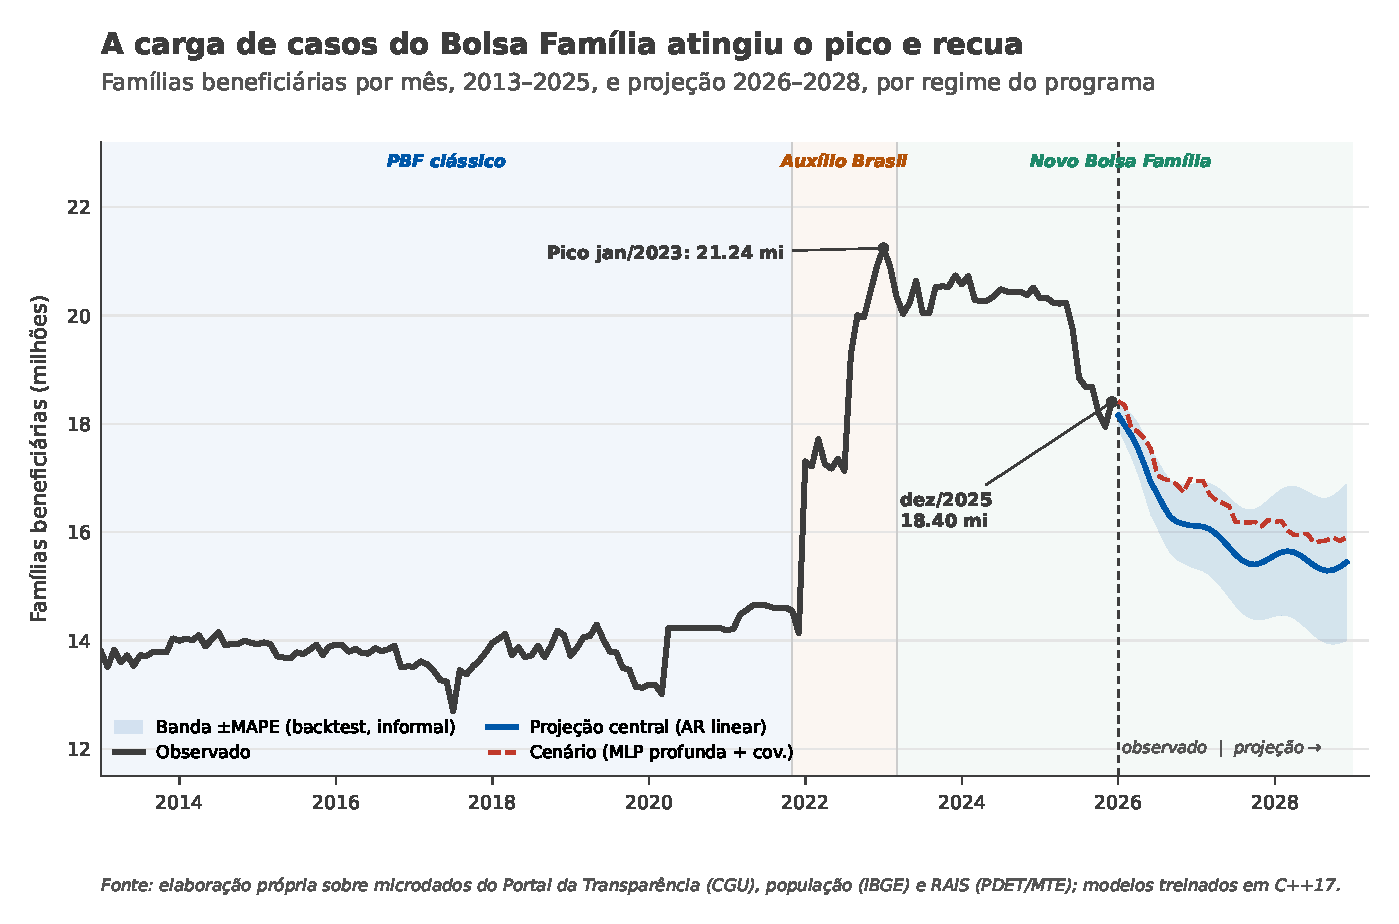
\includegraphics[width=0.97\textwidth]{fig01_serie_nacional.pdf}
\caption{\textbf{Carga de casos nacional, 2013\textendash 2025, e projeção
2026\textendash 2028, por regime do programa.} A série atingiu o pico em
2022\textendash 2023 e recua. A projeção central indica consolidação em
torno de 15,4 milhões de famílias até 2028. A banda sombreada é o intervalo
de 95\% derivado do MAPE agregado de backtest.}
\label{fig:serie}
\end{figure}

\begin{table}[H]
\centering
\caption{Marcos da carga de casos nacional}
\label{tab:projecao}
\small
\begin{tabular}{@{}lr@{}}
\toprule
\textbf{Grandeza} & \textbf{Valor (famílias)} \\
\midrule
Pico (jan/2023)                                  & \num{21243010} \\
Último observado (dez/2025)                        & \num{18401764} \\
Projeção central (AR linear), dez/2028            & $\approx$ \num{15442971} \\
AR linear + cov., dez/2028                         & $\approx$ \num{15456747} \\
MLP profunda + cov., dez/2028                       & $\approx$ \num{15902025} \\
Banda de 95\% em dez/2028                           & $[\,\num{13999098};\ \num{16886844}\,]$ \\
\bottomrule
\end{tabular}
\par\smallskip
{\footnotesize Banda nacional de $\pm$MAPE de backtest, de 1,3\% (curto) a
9,4\% (dez/2028). Fonte: elaboração própria.}
\end{table}

\subsection{Leitura fiscal}

A implicação é direta. Pela equação~\eqref{eq:custo}, com a carga de casos
plana ou declinante, o custo futuro é governado pela \emph{alavanca de
política} \textemdash{} o valor do benefício \textemdash{}, não por uma
demanda em expansão. A parcela \emph{estrutural} do gasto não cresce;
eventuais aumentos de custo serão, sob a hipótese de ausência de novo
choque institucional, escolhas discricionárias de benefício. E, porque o
agregado nacional é previsível com erro inferior a 4,7\% em doze meses
(e ainda menor com covariáveis), essa parcela pode ser planejada com folga
adequada ao ciclo orçamentário.

\subsection{Do caseload ao custo: como usar a projeção}

A projeção é um insumo, não uma resposta final. A equação~\eqref{eq:custo}
sugere o procedimento de uso. Tomada a trajetória central da carga de
casos $\widehat{N}_t$ e sua banda
$[\,\widehat{N}_t^{\,\text{lo}},\,\widehat{N}_t^{\,\text{hi}}\,]$, o custo
projetado em $t$ é $\widehat{C}_t\approx \widehat{N}_t\cdot \bar{b}_t$, onde
$\bar{b}_t$ é o benefício médio \textemdash{} uma escolha de política. A
incerteza do custo decompõe-se, então, em duas fontes \emph{ortogonais}: a
incerteza \emph{estrutural} (a banda da carga de casos, que este artigo
quantifica em ${<}9{,}4\%$ até 2028) e a incerteza \emph{de política} (o
valor do benefício, que o gestor controla). Separá-las é o ganho
prático: o planejador pode tratar a primeira como dado \textemdash{}
estreito e previsível \textemdash{} e concentrar a deliberação na segunda,
que é onde residem tanto a escolha quanto o grosso da variação possível do
gasto. A projeção, portanto, não substitui a decisão orçamentária; ela
\emph{delimita} a parte da conta que não está em disputa, tornando
explícita a parte que está. É essa delimitação, e não um número único de
gasto, o produto de política deste trabalho.

% =====================================================================
\section{Limitações}
\label{sec:limitacoes}
% =====================================================================

A honestidade do exercício exige enumerar suas fronteiras.

\textbf{1. Reversão à média na recursão.} A projeção recursiva de múltiplos
anos arrasta as previsões à média histórica de cada município; formulações
diretas de múltiplos horizontes, ou estado de espaço com tendência
amortecida~\C{ref:hyndman}, mitigariam o efeito.

\textbf{2. Covariáveis congeladas no futuro.} Na projeção, população e
emprego formal são mantidos em 2024. Acoplar projeções demográficas
oficiais do IBGE e cenários de emprego refinaria o longo prazo
\textemdash{} justamente onde as covariáveis mais importam.

\textbf{3. Choques de política exógenos.} Um quarto regime institucional
não é previsível do histórico; as previsões são condicionais a ``nenhum
novo choque''. É limitação intrínseca de modelos sem variáveis de política.

\textbf{4. Frequência das covariáveis.} População e RAIS são anuais e
publicadas com defasagem; sua granularidade temporal grosseira limita o
ganho a curto prazo (Seção~\ref{sec:efeito}). Séries mensais de mercado de
trabalho (p.\ ex.\ CAGED) poderiam estender o benefício a horizontes
intermediários.

\textbf{5. Cobertura da agregação.} A trajetória nacional soma os
municípios com janela final completa e covariáveis ($\approx 99\%$); a
exclusão dos 29 municípios sem casamento de código introduz viés de
cobertura desprezível, mas não nulo.

% =====================================================================
\section{Extensões}
\label{sec:extensoes}
% =====================================================================

Três extensões decorrem naturalmente.

\textbf{Mais covariáveis e maior frequência.} Os fluxos de entrada e saída
do Cadastro Único, séries mensais de emprego (CAGED) e indicadores de
informalidade dariam ao modelo \textemdash{} sobretudo ao profundo
\textemdash{} estrutura não-linear adicional a explorar, possivelmente
permitindo à profundidade enfim compensar em horizontes intermediários.

\textbf{Previsões probabilísticas calibradas.} A banda atual é o MAPE de
backtest, substituto razoável porém não calibrado. Regressão
quantílica~\C{ref:koenker} ou predição conforme~\C{ref:conformal}
produziriam intervalos com cobertura teoricamente garantida \textemdash{}
um avanço natural para o uso orçamentário.

\textbf{Heterogeneidade espacial.} A relação cobertura\textendash emprego
(Figura~\ref{fig:cob-emp}) e a desigualdade entre estados
(Figura~\ref{fig:cob-uf}) sugerem que modelos com efeitos regionais,
covariáveis espaciais ou agrupamento por perfil municipal poderiam capturar
dinâmicas locais que o modelo global, por construção, média. Um caminho
natural é hierarquizar a previsão \textemdash{} reconciliar trajetórias
municipais, estaduais e nacional \textemdash{} de modo que a soma das
partes seja coerente com o todo, técnica madura na literatura de previsão
hierárquica.

\textbf{Modelagem explícita de regime.} As três faixas institucionais da
Figura~\ref{fig:serie} são, hoje, tratadas como dadas. Incorporar
indicadores de regime, ou variáveis de política (limiares de elegibilidade,
valor do benefício), permitiria \emph{condicionar} a previsão a cenários de
política \textemdash{} transformando o modelo, de puramente preditivo, em
ferramenta de simulação contrafactual para o gestor. Essa é, em última
análise, a ponte entre a previsão da demanda estrutural, objeto deste
artigo, e a equação de custo~\eqref{eq:custo} que a motiva.

Em conjunto, essas extensões partilham um princípio: cada uma adiciona
\emph{estrutura} que o modelo univariado global não contém. O presente
artigo mostra que a primeira dose de estrutura externa \textemdash{}
demografia e emprego \textemdash{} já paga, e onde paga (horizontes
longos). A pergunta aberta é se doses adicionais, de maior frequência e
granularidade, deslocam enfim a fronteira a favor da profundidade
\textemdash{} ou se a parcimônia continua, como aqui, a usar melhor cada
nova informação.

% =====================================================================
\section{Conclusões}
\label{sec:conclusoes}
% =====================================================================

Seis conclusões emergem.

\textbf{Primeira:} a carga de casos do Bolsa Família \emph{atingiu o pico e
consolida-se} \textemdash{} de $\approx$ 21,2 milhões de famílias em
janeiro de 2023 para 18,4 milhões em dezembro de 2025, com projeção em
torno de 15,4\textendash 15,9 milhões para 2028. A demanda estrutural não
cresce.

\textbf{Segunda:} o \emph{aprendizado supera a ingênua em horizontes de
planejamento} \textemdash{} até 27\% de redução de MAE em seis meses, de
forma robusta \textemdash{}, mas \emph{não} a um mês, quando a série é
quase um passeio aleatório.

\textbf{Terceira:} o \emph{modelo do tamanho certo vence}. A autorregressão
linear domina o perceptron profundo em todo horizonte, mesmo com
covariáveis; a profundidade só ajuda quando regularizada, e ainda assim
fica atrás.

\textbf{Quarta:} as \emph{covariáveis de demografia e emprego carregam
sinal real, cujo valor cresce com o horizonte} \textemdash{} negligíveis ou
prejudiciais a 1\textendash 3 meses, elevam o modelo linear de $+10\%$ para
$+17\%$ de redução de MAE em 12 meses, tornando-o o melhor preditor de
longo prazo.

\textbf{Quinta:} as \emph{previsões nacionais são estreitas} \textemdash{}
MAPE agregado abaixo de 4,7\% em doze meses, e ainda menor com covariáveis
\textemdash{}, adequadas ao planejamento orçamentário, graças ao
cancelamento de erros na agregação.

\textbf{Sexta:} o \emph{custo fiscal é uma escolha de política}, não uma
inevitabilidade conduzida pela carga de casos \textemdash{} o ponto de
maior relevância para o debate de sustentabilidade.

\subsection{Método aberto e o sentido das duas perguntas}

Registra-se, por fim, o valor da abordagem do zero: ao implementar cada
peça à mão em C++17, seguindo Chen e Gupta~\C{ref:chen-gupta}, e ao
reconciliar três bases públicas oficiais em um único painel, o experimento
permanece integralmente auditável. Não há caixa-preta entre os dados
públicos e a conclusão \textemdash{} cada número da Tabela~\ref{tab:acuracia}
pode ser regenerado, e cada figura, reconstruída, a partir do código e dos
artefatos versionados (Seção~\ref{sec:reprod}).

As duas perguntas metodológicas que organizaram o artigo \textemdash{}
\emph{quando a profundidade compensa?} e \emph{quanto valem covariáveis, e
em que horizonte?} \textemdash{} têm, à luz da
equação~\eqref{eq:bv}, a mesma resposta de fundo: o que importa não é a
capacidade do modelo nem a quantidade de informação \emph{em abstrato}, mas
o casamento entre a estrutura do modelo, a estrutura da informação e a
estrutura do problema. A profundidade não compensou porque o sinal é quase
log-linear; as covariáveis compensaram apenas no longo prazo porque é lá
que a autocorrelação se esgota e a estrutura externa passa a importar. Não
há, neste domínio, um almoço grátis: há o ajuste certo entre ferramenta e
tarefa. É uma lição modesta, mas é a que os dados públicos brasileiros, aqui
examinados com rigor, sustentam \textemdash{} e que vale, plausivelmente,
muito além da carga de casos de um único programa social.

% =====================================================================
\newpage
\section*{Apêndice A \textendash{} Métricas completas}
\addcontentsline{toc}{section}{Apêndice A \textendash{} Métricas completas}

A Tabela~\ref{tab:apA} reporta RMSE e $R^2$ dos cinco modelos nos quatro
horizontes, complementando o MAE e o MAPE da Tabela~\ref{tab:acuracia}. O
$R^2$ permanece acima de 0,985 em toda linha \textemdash{} artefato da
enorme variância entre municípios \textemdash{}, reforçando que a métrica
informativa é o MAPE. O RMSE, mais sensível a grandes erros, ordena os
modelos de forma consistente com o MAE: a autorregressão linear (com ou
sem covariáveis) tem o menor RMSE em 3, 6 e 12 meses.

\begin{table}[H]
\centering
\caption{Métricas completas por horizonte e modelo}
\label{tab:apA}
\small
\begin{tabular}{@{}clrr@{}}
\toprule
\textbf{$H$} & \textbf{Modelo} & \textbf{RMSE (fam.)} & \textbf{$R^2$} \\
\midrule
\multirow{5}{*}{1}
 & Persistência & 412 & 0,9992 \\
 & AR linear & 365 & 0,9994 \\
 & MLP profunda & 379 & 0,9993 \\
 & AR linear + cov. & 507 & 0,9988 \\
 & MLP profunda + cov. & 395 & 0,9993 \\
\midrule
\multirow{5}{*}{3}
 & Persistência & 797 & 0,9970 \\
 & AR linear & 574 & 0,9984 \\
 & MLP profunda & 784 & 0,9971 \\
 & AR linear + cov. & 796 & 0,9970 \\
 & MLP profunda + cov. & 958 & 0,9956 \\
\midrule
\multirow{5}{*}{6}
 & Persistência & 1.313 & 0,9917 \\
 & AR linear & 805 & 0,9969 \\
 & MLP profunda & 1.300 & 0,9919 \\
 & AR linear + cov. & 805 & 0,9969 \\
 & MLP profunda + cov. & 1.302 & 0,9919 \\
\midrule
\multirow{5}{*}{12}
 & Persistência & 1.684 & 0,9864 \\
 & AR linear & 1.171 & 0,9934 \\
 & MLP profunda & 1.538 & 0,9887 \\
 & AR linear + cov. & 1.183 & 0,9933 \\
 & MLP profunda + cov. & 1.642 & 0,9871 \\
\bottomrule
\end{tabular}
\par\smallskip
{\footnotesize Fonte: elaboração própria.}
\end{table}

\newpage
\section*{Apêndice B \textendash{} Comparações pareadas completas}
\addcontentsline{toc}{section}{Apêndice B \textendash{} Comparações pareadas completas}

A Tabela~\ref{tab:apB} reporta todas as seis comparações pareadas de
interesse nos quatro horizontes: cada modelo aprendido contra a
persistência e entre si, e os dois testes de covariável. Todos os
valores-$p$ de Wilcoxon são inferiores a $10^{-4}$ (em geral
$<10^{-30}$); dado $n\approx\num{66504}$, a leitura relevante está no
intervalo de confiança (estritamente positivo $\Rightarrow$ vantagem
robusta) e na taxa de vitória.

\begin{table}[H]
\centering
\caption{Comparações pareadas completas ($\Delta$MAE${}>0$ favorece o primeiro modelo)}
\label{tab:apB}
\small
\begin{tabular}{@{}clrcr@{}}
\toprule
\textbf{$H$} & \textbf{Comparação} & \textbf{$\Delta$MAE} & \textbf{IC 95\%} & \textbf{Vit.\ (\%)} \\
\midrule
\multirow{6}{*}{1}
 & AR linear vs persist. & $-2{,}9$ & $[-4{,}7;\,-1{,}2]$ & 48,3 \\
 & MLP prof. vs persist. & $-0{,}3$ & $[-1{,}8;\,+1{,}1]$ & 49,5 \\
 & AR linear vs MLP prof. & $-2{,}6$ & $[-4{,}1;\,-1{,}1]$ & 48,0 \\
 & AR lin.+cov vs AR linear & $-2{,}8$ & $[-5{,}4;\,-0{,}3]$ & 51,1 \\
 & MLP+cov vs MLP prof. & $-0{,}5$ & $[-1{,}6;\,+0{,}5]$ & 52,1 \\
 & MLP+cov vs AR linear & $+2{,}1$ & $[+0{,}5;\,+3{,}5]$ & 53,0 \\
\midrule
\multirow{6}{*}{3}
 & AR linear vs persist. & $+20{,}2$ & $[+17{,}6;\,+22{,}7]$ & 58,5 \\
 & MLP prof. vs persist. & $+0{,}8$ & $[-1{,}6;\,+3{,}2]$ & 53,1 \\
 & AR linear vs MLP prof. & $+19{,}4$ & $[+16{,}8;\,+22{,}0]$ & 56,1 \\
 & AR lin.+cov vs AR linear & $-9{,}8$ & $[-12{,}4;\,-7{,}2]$ & 52,9 \\
 & MLP+cov vs MLP prof. & $-7{,}7$ & $[-10{,}4;\,-5{,}2]$ & 50,6 \\
 & MLP+cov vs AR linear & $-27{,}1$ & $[-31{,}6;\,-23{,}2]$ & 44,1 \\
\midrule
\multirow{6}{*}{6}
 & AR linear vs persist. & $+56{,}0$ & $[+49{,}7;\,+62{,}4]$ & 64,2 \\
 & MLP prof. vs persist. & $+4{,}3$ & $[+0{,}5;\,+8{,}0]$ & 56,4 \\
 & AR linear vs MLP prof. & $+51{,}7$ & $[+46{,}5;\,+57{,}3]$ & 61,5 \\
 & AR lin.+cov vs AR linear & $-0{,}8$ & $[-2{,}1;\,+0{,}5]$ & 53,2 \\
 & MLP+cov vs MLP prof. & $+12{,}7$ & $[+8{,}4;\,+16{,}7]$ & 59,2 \\
 & MLP+cov vs AR linear & $-39{,}0$ & $[-44{,}7;\,-33{,}6]$ & 41,4 \\
\midrule
\multirow{6}{*}{12}
 & AR linear vs persist. & $+25{,}7$ & $[+14{,}2;\,+37{,}9]$ & 56,9 \\
 & MLP prof. vs persist. & $-28{,}3$ & $[-36{,}7;\,-19{,}6]$ & 56,3 \\
 & AR linear vs MLP prof. & $+54{,}1$ & $[+47{,}7;\,+61{,}3]$ & 57,9 \\
 & AR lin.+cov vs AR linear & $+19{,}8$ & $[+12{,}1;\,+27{,}5]$ & 54,5 \\
 & MLP+cov vs MLP prof. & $-1{,}5$ & $[-5{,}9;\,+3{,}1]$ & 54,6 \\
 & MLP+cov vs AR linear & $-55{,}6$ & $[-64{,}1;\,-47{,}6]$ & 45,5 \\
\bottomrule
\end{tabular}
\par\smallskip
{\footnotesize IC por bootstrap pareado (\num{2000} reamostragens). Fonte:
elaboração própria.}
\end{table}

% =====================================================================
\newpage
\section*{Referências}
\addcontentsline{toc}{section}{Referências}
\setcounter{mref}{0}

\begin{singlespace}

\refentry{ref:lei-pbf}
BRASIL. \textbf{Lei n.\textsuperscript{o} 10.836, de 9 de janeiro de
2004}. Cria o Programa Bolsa Família. Diário Oficial da União, Brasília,
2004. Disponível em:
\url{https://www.planalto.gov.br/ccivil_03/_ato2004-2006/2004/lei/l10.836.htm}.
Acesso em: 22 jun.\ 2026.

\refentry{ref:lei-ab}
BRASIL. \textbf{Lei n.\textsuperscript{o} 14.284, de 29 de dezembro de
2021}. Institui o Programa Auxílio Brasil. Diário Oficial da União,
Brasília, 2021. Disponível em:
\url{https://www.planalto.gov.br/ccivil_03/_ato2019-2022/2021/lei/l14284.htm}.
Acesso em: 22 jun.\ 2026.

\refentry{ref:lei-nbf}
BRASIL. \textbf{Lei n.\textsuperscript{o} 14.601, de 19 de junho de
2023}. Institui o Programa Bolsa Família. Diário Oficial da União,
Brasília, 2023. Disponível em:
\url{https://www.planalto.gov.br/ccivil_03/_ato2023-2026/2023/lei/l14601.htm}.
Acesso em: 22 jun.\ 2026.

\refentry{ref:portal-transparencia}
CONTROLADORIA-GERAL DA UNIÃO (CGU). \textbf{Portal da Transparência do
Governo Federal: Bolsa Família e Auxílio Brasil}. Brasília: CGU.
Disponível em:
\url{https://portaldatransparencia.gov.br/beneficios/bolsa-familia}.
Acesso em: 22 jun.\ 2026.

\refentry{ref:ibge-pop}
INSTITUTO BRASILEIRO DE GEOGRAFIA E ESTATÍSTICA (IBGE). \textbf{Estimativas
da população residente para os municípios e para as unidades da
federação}. Rio de Janeiro: IBGE. Disponível em:
\url{https://www.ibge.gov.br/estatisticas/sociais/populacao/9103-estimativas-de-populacao.html}.
Acesso em: 22 jun.\ 2026.

\refentry{ref:rais}
BRASIL. Ministério do Trabalho e Emprego (MTE). \textbf{Relação Anual de
Informações Sociais (RAIS)}. Programa de Disseminação das Estatísticas do
Trabalho (PDET). Brasília: MTE. Disponível em:
\url{https://www.gov.br/trabalho-e-emprego/pt-br/assuntos/estatisticas-trabalho/rais}.
Acesso em: 22 jun.\ 2026.

\refentry{ref:chen-gupta}
CHEN, Bill; GUPTA, Vikash. \textbf{Deep Learning with C++: Design and
deploy neural networks using CUDA for high-performance AI in C++}.
Birmingham: Packt Publishing, 2026. ISBN 978-1-83588-002-9.

\refentry{ref:goodfellow}
GOODFELLOW, Ian; BENGIO, Yoshua; COURVILLE, Aaron. \textbf{Deep Learning}.
Cambridge, MA: MIT Press, 2016. Disponível em:
\url{https://www.deeplearningbook.org}. Acesso em: 22 jun.\ 2026.

\refentry{ref:lecun}
LECUN, Yann; BENGIO, Yoshua; HINTON, Geoffrey. Deep learning.
\textbf{Nature}, v. 521, p. 436\textendash 444, 2015.
DOI: 10.1038/nature14539.

\refentry{ref:rumelhart}
RUMELHART, David E.; HINTON, Geoffrey E.; WILLIAMS, Ronald J. Learning
representations by back-propagating errors. \textbf{Nature}, v. 323,
p. 533\textendash 536, 1986. DOI: 10.1038/323533a0.

\refentry{ref:cybenko}
CYBENKO, George. Approximation by superpositions of a sigmoidal function.
\textbf{Mathematics of Control, Signals and Systems}, v. 2, n. 4,
p. 303\textendash 314, 1989. DOI: 10.1007/BF02551274.

\refentry{ref:hornik}
HORNIK, Kurt; STINCHCOMBE, Maxwell; WHITE, Halbert. Multilayer feedforward
networks are universal approximators. \textbf{Neural Networks}, v. 2,
n. 5, p. 359\textendash 366, 1989. DOI: 10.1016/0893-6080(89)90020-8.

\refentry{ref:he}
HE, Kaiming; ZHANG, Xiangyu; REN, Shaoqing; SUN, Jian. Delving deep into
rectifiers: surpassing human-level performance on ImageNet classification.
In: \textbf{IEEE International Conference on Computer Vision (ICCV)}, 2015.
arXiv:1502.01852.

\refentry{ref:glorot}
GLOROT, Xavier; BENGIO, Yoshua. Understanding the difficulty of training
deep feedforward neural networks. In: \textbf{AISTATS}, 2010. v. 9,
p. 249\textendash 256.

\refentry{ref:adam}
KINGMA, Diederik P.; BA, Jimmy. Adam: a method for stochastic optimization.
In: \textbf{International Conference on Learning Representations (ICLR)},
2015. arXiv:1412.6980.

\refentry{ref:adamw}
LOSHCHILOV, Ilya; HUTTER, Frank. Decoupled weight decay regularization.
In: \textbf{ICLR}, 2019. arXiv:1711.05101.

\refentry{ref:box-jenkins}
BOX, George E. P.; JENKINS, Gwilym M. \textbf{Time Series Analysis:
Forecasting and Control}. San Francisco: Holden-Day, 1970.

\refentry{ref:hyndman}
HYNDMAN, Rob J.; ATHANASOPOULOS, George. \textbf{Forecasting: Principles
and Practice}. 3. ed. Melbourne: OTexts, 2021. Disponível em:
\url{https://otexts.com/fpp3/}. Acesso em: 22 jun.\ 2026.

\refentry{ref:hyndman-koehler}
HYNDMAN, Rob J.; KOEHLER, Anne B. Another look at measures of forecast
accuracy. \textbf{International Journal of Forecasting}, v. 22, n. 4,
p. 679\textendash 688, 2006. DOI: 10.1016/j.ijforecast.2006.03.001.

\refentry{ref:bergmeir}
BERGMEIR, Christoph; BENÍTEZ, José M. On the use of cross-validation for
time series predictor evaluation. \textbf{Information Sciences}, v. 191,
p. 192\textendash 213, 2012. DOI: 10.1016/j.ins.2011.12.028.

\refentry{ref:m4}
MAKRIDAKIS, Spyros; SPILIOTIS, Evangelos; ASSIMAKOPOULOS, Vassilios. The
M4 Competition: 100,000 time series and 61 forecasting methods.
\textbf{International Journal of Forecasting}, v. 36, n. 1,
p. 54\textendash 74, 2020. DOI: 10.1016/j.ijforecast.2019.04.014.

\refentry{ref:hewamalage}
HEWAMALAGE, Hansika; BERGMEIR, Christoph; BANDARA, Kasun. Global models for
time series forecasting: a simulation study. \textbf{Pattern Recognition},
v. 124, 108441, 2022. DOI: 10.1016/j.patcog.2021.108441.

\refentry{ref:smyl}
SMYL, Slawek. A hybrid method of exponential smoothing and recurrent neural
networks for time series forecasting. \textbf{International Journal of
Forecasting}, v. 36, n. 1, p. 75\textendash 85, 2020.
DOI: 10.1016/j.ijforecast.2019.03.017.

\refentry{ref:salinas}
SALINAS, David; FLUNKERT, Valentin; GASTHAUS, Jan; JANUSCHOWSKI, Tim.
DeepAR: probabilistic forecasting with autoregressive recurrent networks.
\textbf{International Journal of Forecasting}, v. 36, n. 3,
p. 1181\textendash 1191, 2020. DOI: 10.1016/j.ijforecast.2019.07.001.

\refentry{ref:lim}
LIM, Bryan; ZOHREN, Stefan. Time-series forecasting with deep learning: a
survey. \textbf{Philosophical Transactions of the Royal Society A},
v. 379, n. 2194, 20200209, 2021. DOI: 10.1098/rsta.2020.0209.

\refentry{ref:dama}
DAMA INTERNATIONAL. \textbf{DAMA-DMBOK: Data Management Body of Knowledge}.
2. ed. Basking Ridge: Technics Publications, 2017.
ISBN 978-1-63462-234-9.

\refentry{ref:spark}
ZAHARIA, Matei; XIN, Reynold S.; WENDELL, Patrick \emph{et al.} Apache
Spark: a unified engine for big data processing. \textbf{Communications of
the ACM}, v. 59, n. 11, p. 56\textendash 65, 2016.
DOI: 10.1145/2934664.

\refentry{ref:delta}
ARMBRUST, Michael; DAS, Tathagata; SUN, Liwen \emph{et al.} Delta Lake:
high-performance ACID table storage over cloud object stores.
\textbf{Proceedings of the VLDB Endowment}, v. 13, n. 12,
p. 3411\textendash 3424, 2020. DOI: 10.14778/3415478.3415560.

\refentry{ref:databricks}
DATABRICKS. \textbf{Databricks Free Edition}. San Francisco: Databricks,
2025. Disponível em: \url{https://www.databricks.com/learn/free-edition}.
Acesso em: 22 jun.\ 2026.

\refentry{ref:medallion}
DATABRICKS. \textbf{What is the medallion lakehouse architecture?}
Documentação técnica. San Francisco: Databricks. Disponível em:
\url{https://www.databricks.com/glossary/medallion-architecture}.
Acesso em: 22 jun.\ 2026.

\refentry{ref:diebold}
DIEBOLD, Francis X.; MARIANO, Roberto S. Comparing predictive accuracy.
\textbf{Journal of Business \& Economic Statistics}, v. 13, n. 3,
p. 253\textendash 263, 1995. DOI: 10.1080/07350015.1995.10524599.

\refentry{ref:wilcoxon}
WILCOXON, Frank. Individual comparisons by ranking methods.
\textbf{Biometrics Bulletin}, v. 1, n. 6, p. 80\textendash 83, 1945.
DOI: 10.2307/3001968.

\refentry{ref:efron}
EFRON, Bradley. Bootstrap methods: another look at the jackknife.
\textbf{The Annals of Statistics}, v. 7, n. 1, p. 1\textendash 26, 1979.
DOI: 10.1214/aos/1176344552.

\refentry{ref:koenker}
KOENKER, Roger; BASSETT, Gilbert. Regression quantiles.
\textbf{Econometrica}, v. 46, n. 1, p. 33\textendash 50, 1978.
DOI: 10.2307/1913643.

\refentry{ref:conformal}
SHAFER, Glenn; VOVK, Vladimir. A tutorial on conformal prediction.
\textbf{Journal of Machine Learning Research}, v. 9, p. 371\textendash 421,
2008.

\end{singlespace}

\end{document}
